%
% Nishat Anjum Khan, MS thesis, 2017
%

% save \@xfloat (modified by uicthesi class)
\makeatletter
\let\orig@xfloat\@xfloat
\makeatother

% UIC thesis template
\documentclass{uicthesi}

% restore \@xfloat and reset baselinestretch in another way
% (thanks to: http://www.latex-community.org/forum/viewtopic.php?f=45&t=20816)
\usepackage{etoolbox}
\makeatletter
\let\@xfloat\orig@xfloat
\patchcmd{\@xfloat}{\columnwidth}{\columnwidth\def\baselinestretch{\@ne}}{}{}
\makeatother

% package for rotating tables sideways
\usepackage{rotating}

% color definitions for TRR12's table
\usepackage[table]{xcolor}
\definecolor{tableShade}{HTML}{e8e8e8}

%\usepackage{enumerate}

% package for using multi-part figures
\usepackage{subfigure}
%\usepackage{subfig}
%\usepackage{graphicx}

% package for aligning equations
\usepackage{amsmath}

% package for providing line-breakable underlining
\usepackage{ulem}

\usepackage{url}
\usepackage{tabularx}


\title{Multi-Sensor Preprocessing for Traffic Light Detection}
\author{Nishat Anjum Khan}
\pdegrees{B.S., Bangladesh University of Engineering and Technology, 2014}
\degree{Master of Science in Electrical and Computer Engineering}
\committee{Rashid Ansari, Chair and Advisor\\Ahmet Enis Cetin, Co-Advisor\\Mojtaba Soltanalian}

\begin{document}
\maketitle


\newcommand{\todo}[1]{\textcolor{blue}{TODO: #1}}
\newcommand{\warn}[1]{\textcolor{red}{WARNING: #1}}
\newcommand{\note}[1]{\textcolor{red}{NOTE: #1}}


\copyrightpage

\dedication

{\null\vfil
{\large
\begin{center}
\textit{To my parents}
\end{center}}
\vfil\null}

\acknowledgements

First, I would like to thank my advisor Dr. Rashid Ansari, for his continuous support and guidance throughout my research and writing of this thesis.  
His feedback and hard questions throughout the dissertation writing helped me to widen my research perspectives.  

I would also like to thank my committee members Dr. Ahmet Enis Cetin and Dr. Mojtaba Soltanalian for their insightful comments and reviewing my work.

Thanks to all of my lab-mates, especially Lubna for all of the fun we have in the last two years. 

Thanks to my parents Md. Muhiuddin Khan, Khaleda Khan, without whose love and support I could never have made it this far. 
Thanks to my brother Khaled Hasan Khan for supporting me throughout this long journey and my life in general.

Last but not least, thanks to my husband Musa for his continuous support and encouragement. This accomplishment would not have been possible without him.


\begin{flushright}
NK
\end{flushright}

%\input{contribution_of_authors}

%\preface
%The preface is purely optional at UIC.

\tableofcontents
\listoftables
\listoffigures


\summary

With the exponential growth of smartphone usage and its computational capability, there is an opportunity today to build a usable navigation system for the visually impaired. 
A smartphone contains virtually all sensors for sensing the surrounding environment such as GPS, cameras, and inertial sensors. 
However, there are many challenges for building a complete navigation system, such as low-level methods of environment sensing, accuracy, and efficient data processing.
In this dissertation, we address some of these challenges and present a system for traffic light detection, which is fundamental for pedestrian navigation by the visually impaired in outdoors. 
In this system, we analyze the video feed from a smartphone's camera using model-based computer vision techniques to detect traffic lights. 
Specifically, we utilize both color and shape information as they are the most prominent features of the traffic lights.
Additionally, we use the inertial sensors of a smartphone to compute the 3D orientation of a smartphone to predict a subpart of a video frame, which is highly probable to contain the traffic lights. 
By processing only that subpart, we improve the computational time by an order of magnitude on average. 
Furthermore, due to the processing of a subpart instead of the whole video frame, our system achieves higher accuracy because of reduced false positive.
Finally, we recognize walk and stop signs for pedestrians in addition to the regular traffic lights to obtain higher confidence during navigation. 
We evaluated this system in various lighting conditions such as cloudy, sunny, and at night, and achieved over 95\% accuracy in the traffic light and sign detection and recognition.



\chapter{Introduction}

We used hough circle \cite{hough_circle} to detect traffic lights.


\chapter{Background}
\label{c:background}
In this chapter we will discuss the background of our system.
The main approch of our system is to improve the traffic light detection using smartphone sensor.
In first part of this chapter we will discuss the inertial sensor of Android and eular angle using sensor fusion.
Later we will discuss the traffic bulb detection process.

\section{Accelerometer}
Accelerometer is one of the motion sensor in smartphone.
Smartphone now a days have three axis accelerometer,which can measure acceleration along this three axis and return a vector in the reference frame.
Accelerometer can not measure free fall acceleration rather it measure the forces that are applied to the sensor itself.
For example, when phone is on the table, it will measure acceleration of g, the acceleration due to gravity, because this is proportional to the accelerometer experienced weight.

Figure \ref{f:acc} shows the reference coordination system of accelerometer in Android phone.
The device measures acceleration ax,ay and az along the three axis of android reference frame.
The acceleration az points towards the outside of screen face, that is perpendicular to the phone plane.
The acceleration ax and ay are along to phone plane.

\begin{figure*}[!ht]
\centering
\subfloat[Accelerator coordination] {\label{f:acc}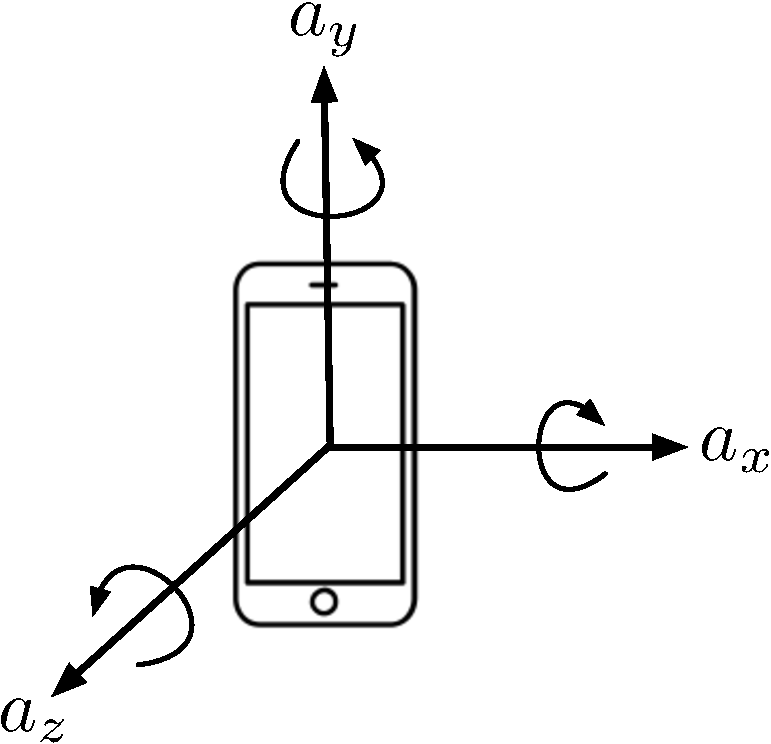
\includegraphics[width=3in]{figures/coord_acceleration.pdf}}
\subfloat[Gyroscope coordination] {\label{f:gyro}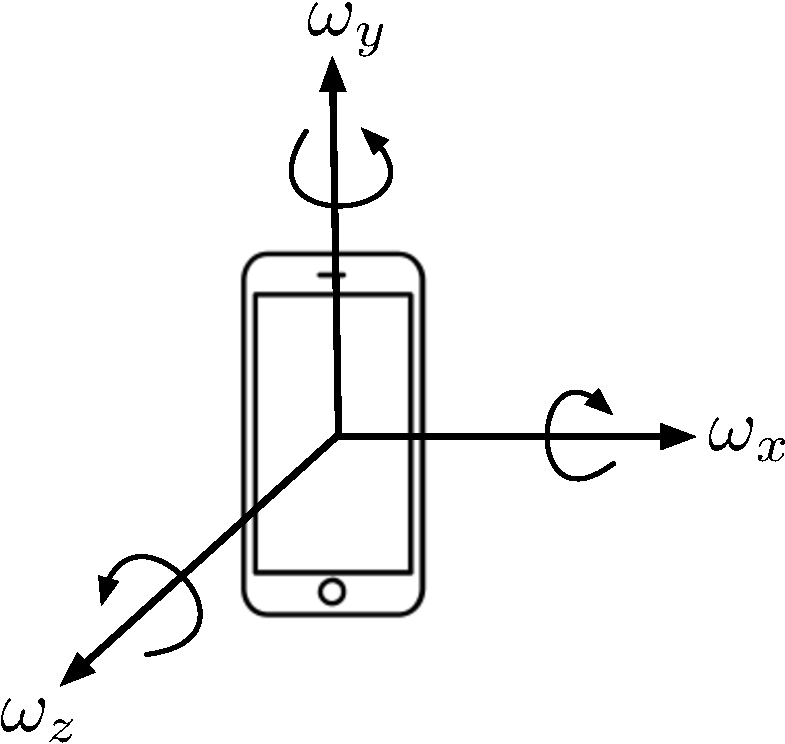
\includegraphics[width=3in]{figures/coord_omega.pdf}}

\caption{Smartphone reference coordination system.}
\label{f:coord_dia}
\end{figure*}

\section{Gyroscope}
Gyroscope measure the rate of rotation or the angular velocity of rotation along the three axis of smartphone's reference frame.
This is also a motion sensor of smartphone like accelerometer.
These gyroscope use MEMS (micro-electro-mechanical sensing) technology, contain vibrating elements to measure Coriolis effect.
When smartphone rotates, there is a change of direction of vibrating elements because of the Coriolis force.
MEMS gyroscope measure these variation along the three axis to estimate the rate of rotation.
Gyroscope output is quite smooth, and very responsive to small rotations.

Figure \ref{f:gyro} shows the reference coordination system of gyroscope in Android phone.
The device measures rate of rotaion wx,wy and wz along the three axis of android reference frame.
The angular velocity of rotation wz points towards the outside of screen face, that is perpendicular to the phone plane, which is the angular velocity of phone's rotaion in X-Y plane.
The rate of rotation wx and wy is along with the phone plane, which is the angular velocity of phone's rotaion in Y-Z plane and Z-X plane respectively.

\section{Geomagnetic field sensor}
Geomagnetic field sensor is a position sensor of smartphone.
It helps to determine the device's physical position in the world's reference frame.
Geomagnetic field sensor mesure the change of magnetioc field and estimates the magnetic field at earth's point to find the declination from the true North.
It provides the geomagnetic field strength along the three coordination axis of refernce frame.


\section{Orientation}
Each sensor defined in previous section has it's own strength and weakness.
Gyroscope is fast, accurate and reliable.
It is very responsive to small rotation so it can track the change of rotation at every timestamp.
But gyroscope data can not measure gravity.
So with accelerometer it can provide a better rotation or motion of the sensor in application's frame reference.
But to have the position of the device in world's reference frame, we need to fused this data with geomagnetic field sensor.
Another motion sensor in android, rotation vector, use this three sensor data to report the orientation of the device in vector form along the axis of reference frame.

This rotation vector provides the axis of the system and the angle of rotation from these axis.
From this angle and axis data, we can get the orientation of the system in terms of pitch, roll and azimuth.

\begin{figure}
\centering
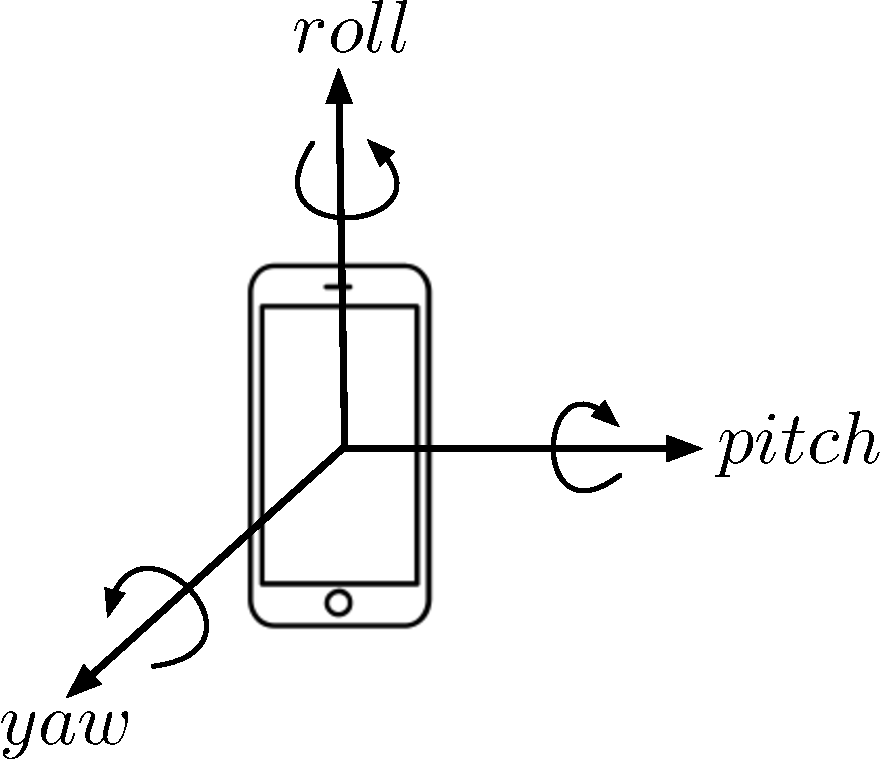
\includegraphics[width=4.2in]{figures/roll_pitch_yaw.pdf}
\caption{Orientation of the smartphone}
\label{f:rpy_dia}
\end{figure}

\ref{f:rpy_dia} shows the orientation of a smartphone about the device's coordination system.
Pitch is the degree of rotation about the X axis.
This is the angle between the plane parallel to device and parallel to the ground.
If device top edge incle to the ground the pitch will be positive and vice versa.
The range of pitch value is -180 degrees to 180 degrees.
Roll is the degree of rotation abot Y axix.
This is the angle between the plane perpendicular to device and perpendicular to ground.
If device's left edge inclenes to the ground roll value is positive.
The range of roll value is -90 degrees to 90 degrees.
Azimuth is the degree of rotation about Z axis.
If the device is faced to the earth's North the azimuth is 0 degree.
Azimuth is 90 degree at earth's East, 180 degree to earth's South and 270 degree to earth's West.

\section {Image Processing}

\subsection{Color Space}
The main two color spaces for processing the color vision are RGB color space and HSV color space.
RGB is a additive color space.
RGB color space describes colors with the amount of red, green and blue color presents on that frame.


\ref{f:rgb} shows the model of RGB space.
It shows that any color of this cube is made of red,blue, and green color.

HSV color space is similar to the way human sees the color.
But RGB defines color in relation to the primary colors.
HSV color space describes color in terms of Hue, Saturation and Value.
It separates the color information from the intensity or the brightness.
Hue is the continuous representation of color type.
In HSV, hue is an angle from 0 to 360 degree. 
But since OpenCv can process data from 0 to 255, so in OpenCv the range is halved.
Every color can be discrimated with the different range of Hue.
Saturation represents the vibracy of the color.
The ranges for saturation is 0 to 255.
The lower saturation meaning gray is present in the color, higher saturation represents primary color.
Value represents brightness of the color.
The range of value is same as saturation, 0 to 255.
Lower value means less bright color, 0 brightness represents black color.

\begin{figure}[htbp]
\begin{minipage}[t]{0.45\linewidth}
    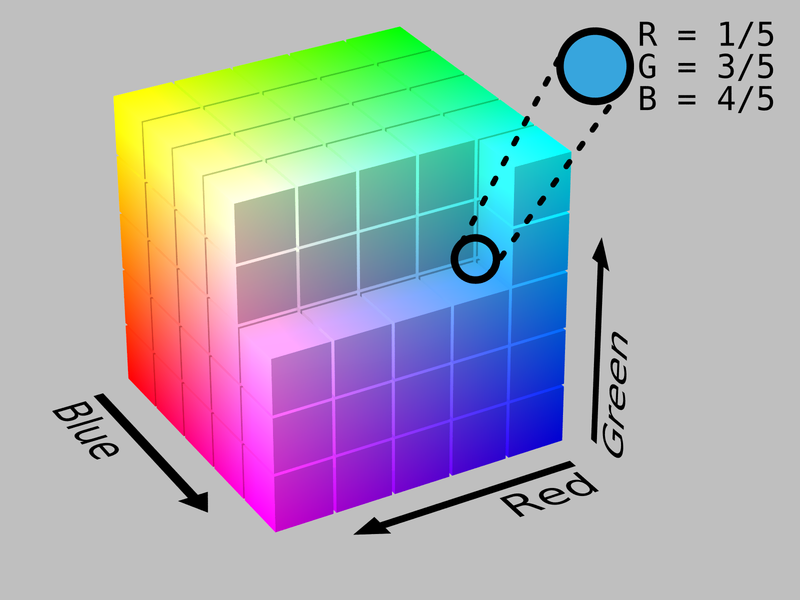
\includegraphics[width=\linewidth]{images/RGB.png}
    \caption{RGB color space}
    \label{f:rgb}
\end{minipage}
    \hfill
\begin{minipage}[t]{0.45\linewidth}
    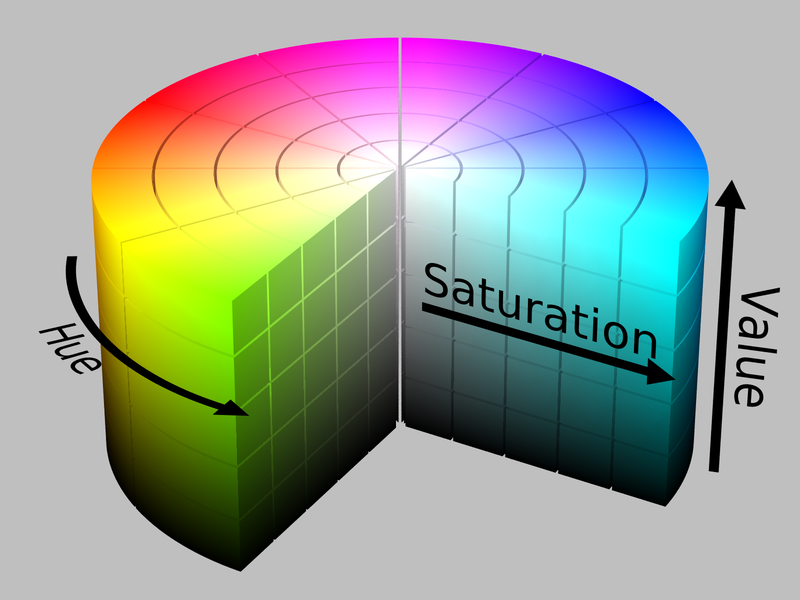
\includegraphics[width=\linewidth]{images/HSV.png}
    \caption{HSV color space}
    \label{f:hsv}
\end{minipage} 
\end{figure}

\ref{f:hsv} shows the cylindrical model of HSV color space.
The Hue is the circular part.
The radious of this circular part represent Saturation and the height is the Value.

\subsection{Hough Circle Transform}
Our system detects the traffic bulb using the hough circle algorithm \cite{houghcir_alg}.
To detect the circle first process is to find the edges in the input image.
The hough circle algotithm uses canny operation for the edge detection.
At every edge pixel, it generates a circle.
An accumulator matrix is created to find the intersection of these circles.
If circle passes through the grid of the accumulator matrix, it increase the coting number of the grid.
The psition of the local maxima of this accumulator matrix provides the corresponding circles centers.








\chapter{Related Work}
\label{c:relw}

In this section, we describe a brief introduction to the most notable research on the navigation for visually impaired.
Visually impaired people can not have information about their location or the direction with respect to the obstacles on the way.
The conventional ways of the guide dog and long cane can help to find out the obstacles on the way, but do not provide their position information.
Navigation systems help people to travel independently.

There has been a significant research \cite{survey} in localization and obstacle avoidance.
For obstacle avoidance, People Sensor \cite{peoplesensor} used pyroelectric and ultrasound sensor to detect an object the user's path.
%It helps to reduce the embarrassment through unintended contact with people and object in the directional path.
\todo{cite more about obstacle}
or virtual blind cane to detect obstacles using laser and inertial measurement unit (IMU) \cite {virtual}

%In this work, we build a navigation system to detect the traffic light in a public street for visually impaired.
%There has some existing systems for helping the blind and visually impaired find their way at indoor and outdoor.
After the introduction of Global Positioning System (GPS) at the 1980s, many systems integrated GPS for the navigation by the visually impaired.
Loomis at el. \cite{loomis1,loomis,loomis2} was one of the first to propose a navigation system using DGPS and correction data over FM to obtain accurate localization.

There are some commercial systems for outdoor navigation for blind and visually impaired users.
Ariadne GPS \cite{arigps} developed by Ciaffoni is one of the first GPS apps for navigation by the blind and visually impaired.
Some other commercially released apps for iPhone and Android devices are BlindSquare \cite{blindsq} and ViaOpta Nav \cite{viaopta}.
These apps use the GPS to inform users the current location, give an announcement of user points of interest and use open source map to navigate.
Seeing Assistant Move \cite{seeing} is the first app for blind people that lets the user to operate the app through speech commands.
Other systems that use GPS to find the user’s location are MoBic \cite{mobic}, BrailleNote GPS and Trekker \cite{human}. 
BrailleNote GPS is commercially available and provides the user with nearby location names and the distance to the destination along the path. 

The GPS provides good location estimations. 
However, there are several shortcomings of the GPS.
The GPS sensor is ineffective at indoors.
The GPS location error can also be high at urban canyons due to multi-path effect and obstructed view of the sky.
%% Some studies proposed and implemented differential GPS which can provide better accuracy \cite{drishti2,gps}.
%% It is costly and needs fixed ground station, only efficient for outdoors.
%% Furthermore, the GPS signal can not be tracked when blind people move through tall buildings or high walls or trees.

Since GPS does not work in indoors, there has been other approaches for localization in indoors using various instrumentation techniques. 
Researchers instrumented indoor areas with ultrasound \cite{drishti} or radio frequency identification (RFID) \cite{rfid} transponders to provide localization with triangulation.
Recently, due to the pervasive deployment of Wi-Fi networks, localization through Wi-Fi triangulation also became popular.  
Most of the localization techniques in indoors using instrumentation depends on fingerprinting where the error can be high.
Furthermore, small changes of the environment can reduce the accuracy.

In order to be extensively applicable, navigation systems needs to be highly accurate.
Additionally, the system needs to be wearable and low cost.
%To achieve this aim we propose a computer vision based navigation system for visually impaired.
To achieve this goal, there has been some recent work on vision based localization with smartphones or other wearable cameras and sensors.
\todo{cite vision based systems w/o map first}
The map based navigation methods \cite{online,map,map2} require a global map to make a decision for the navigation. 
In map-based localization systems, sequential images of the environment are registered in a database.
Then to obtain the location and orientation in the same area at a later time images are matched in the database.
In \cite{fly,fly2,fly3}, Simultaneous Localization and Mapping is used to create a map while moving along with the localization.
In \cite{visual}, the authors proposed a system with a wearable stereo camera for higher accuracy localization utilizing the depth information.

In outdoor streets, traffic light detection is an important part of the navigation system for the visually impaired.
There has been significant research on traffic light detection for autonomous driving and driving assistance systems \cite{traffic_turan,selfdrive,traffic,traffic2,traffic3}.
In \cite{traffic_turan}, the authors combined previously mapped traffic light locations along with the vehicle location to achieve reliable estimation of traffic light status.
In recent years, in addition to the model-based methods \cite{model,model2}, learning-based methods \cite{survey_traffic} became popular for traffic light detection.
The model-based approaches create a heuristic model that rely on color or shape information.
%These approves were dominant in the past decade.
The color information is significant for traffic light detection.
%Primarily to find the region of interest (ROI) and to classify the traffic light state we use the color information.
The model-based systems usually define a heuristic threshold for color to distinguish the traffic lights from the surroundings in a selected color space.
The RGB color space is the most common as the input video frames are in this space \cite{rgb2}.
However, in RGB color space, the color and intensity information is mixed in all the channels, as we discussed in \S\ref{s:color_space}.
As a result, the values of RGB change in different lightening condition.
Alternatively, the HSV color space is more immune to lightening condition and the hue distribution is different for each color unlike the RGB space.
In recent years, most of the research in traffic light detection used HSV space \cite{hsv2}.
To make the model-based approach  more robust, the shape information of traffic light is fused with the color information.
Traffic light's shape can be obtained by applying the Hough transform on an edge map \cite{hough,hough2,signalguru} or by using radial symmetry \cite{radial,radial2}.

Learning-based model \cite{learning,learning2} is another approach to detect traffic lights.
In \cite{selfdrive}, SVM classifier together with HOG features are used for traffic light detection. 
In \cite{acf,acf2,lisa_cvpr}, authors used Aggregated Channel Feature (ACF) for traffic light detection, which resulted in higher accuracy.
Traffic light detection using deep learning is introduced in \cite{cnn,cnn2,cnn3}, where a convolutional neural network (CNN) model detects and recognizes traffic light states using the region of interest information from the smartphone GPS sensor.

%For our system to detect traffic light states, we use the HSV space due to the description of color in HSV space is similar to the human perspective and we use Hough circle transform to get the shape information of the traffic light. 

For outdoor navigation system, traffic light detection is only a part of the end-to-end system for autonomous driving or pedestrian navigation.
These systems also include obstacle detection, cross-walk detection, pedestrian movement detection, and path planning.
Reducing the processing time of individual frames for traffic light detection is important for achiving lower processing time for the entire pipeline.
In general, traffic lights occupy only a subpart of a video frame.
It is possible to reduce the computation time for traffic light detection by only processing that subpart of the frame.
We can utilize the GPS and other intertial sensors (e.g., accelerometer, gyroscope, magnetic field sensor) \cite{sensor,sensor2,sensor3} to predict the change in the camera's viewpoint and infer a subpart of the frame that contains the traffic lights. 
%It is important to use less time to detect the traffic light.
Nowadays, smartphones usage is growing for the navigation purpose since most of the smartphones has built in camera and they are easy to carry around.
Additionally, most of the smartphones contain inertial sensors, which are useful.

For autonomous cars or driving assistance systems, the position of the traffic light is stable with respect to the vehicles.
SignalGuru \cite{signalguru} utlized the intertial sensors in a smartphone to predict the position of the traffic light in the camera's viewpoint.
Since the traffic light is always in the upper part of the frame while driving, they only processed the upper half of the frame for traffic light detection.
In the context of pedestrian navigation, the viewpont of a smartphone's camera is not static because of the body movement \cite{sensor_pedestrian,sensor_pedestrian2}.
Thus, it is more challenging to select a subpart of a frame for traffic light detection.
%% In this case, we can not process a predefined part of the frames.
%% We need to predict the location of the traffic light with the movement and the orientation of the smartphones.
%% In our system, we use the sensor hints at each video frame to get the relative position of traffic light from the previous video frame and finally processed that area to detect the traffic light state.


%% In our system, we use the model-based computer vision technique to detect and recognize the traffic light states.
%% Our main approach is to use the sensor hints to improve the computation time and the misdetection rate.
%% If we adopt these learning based approaches as our detection method with the sensor hint the result can be approved more.  






\chapter{System Architecture}
\label{c:system}
Two major components in our system are: (a) processing of video frames using computer vision techniques to detect traffic lights, and (b) selection of a subpart of a frame using inertial sensor hints to reduce both computation time and spurious detection of traffic lights. 
In this chapter, we present the end-to-end system and describe various components of the system pipeline.

%% In this chapter, we discuss the system overview for traffic light detection.
%% This system detects the color of a traffic light in a recorded video frame.
%% We captured video using a smartphone along with the sensor data.

\section{Overview}
\label{s:overview}


\begin{figure}
\centering
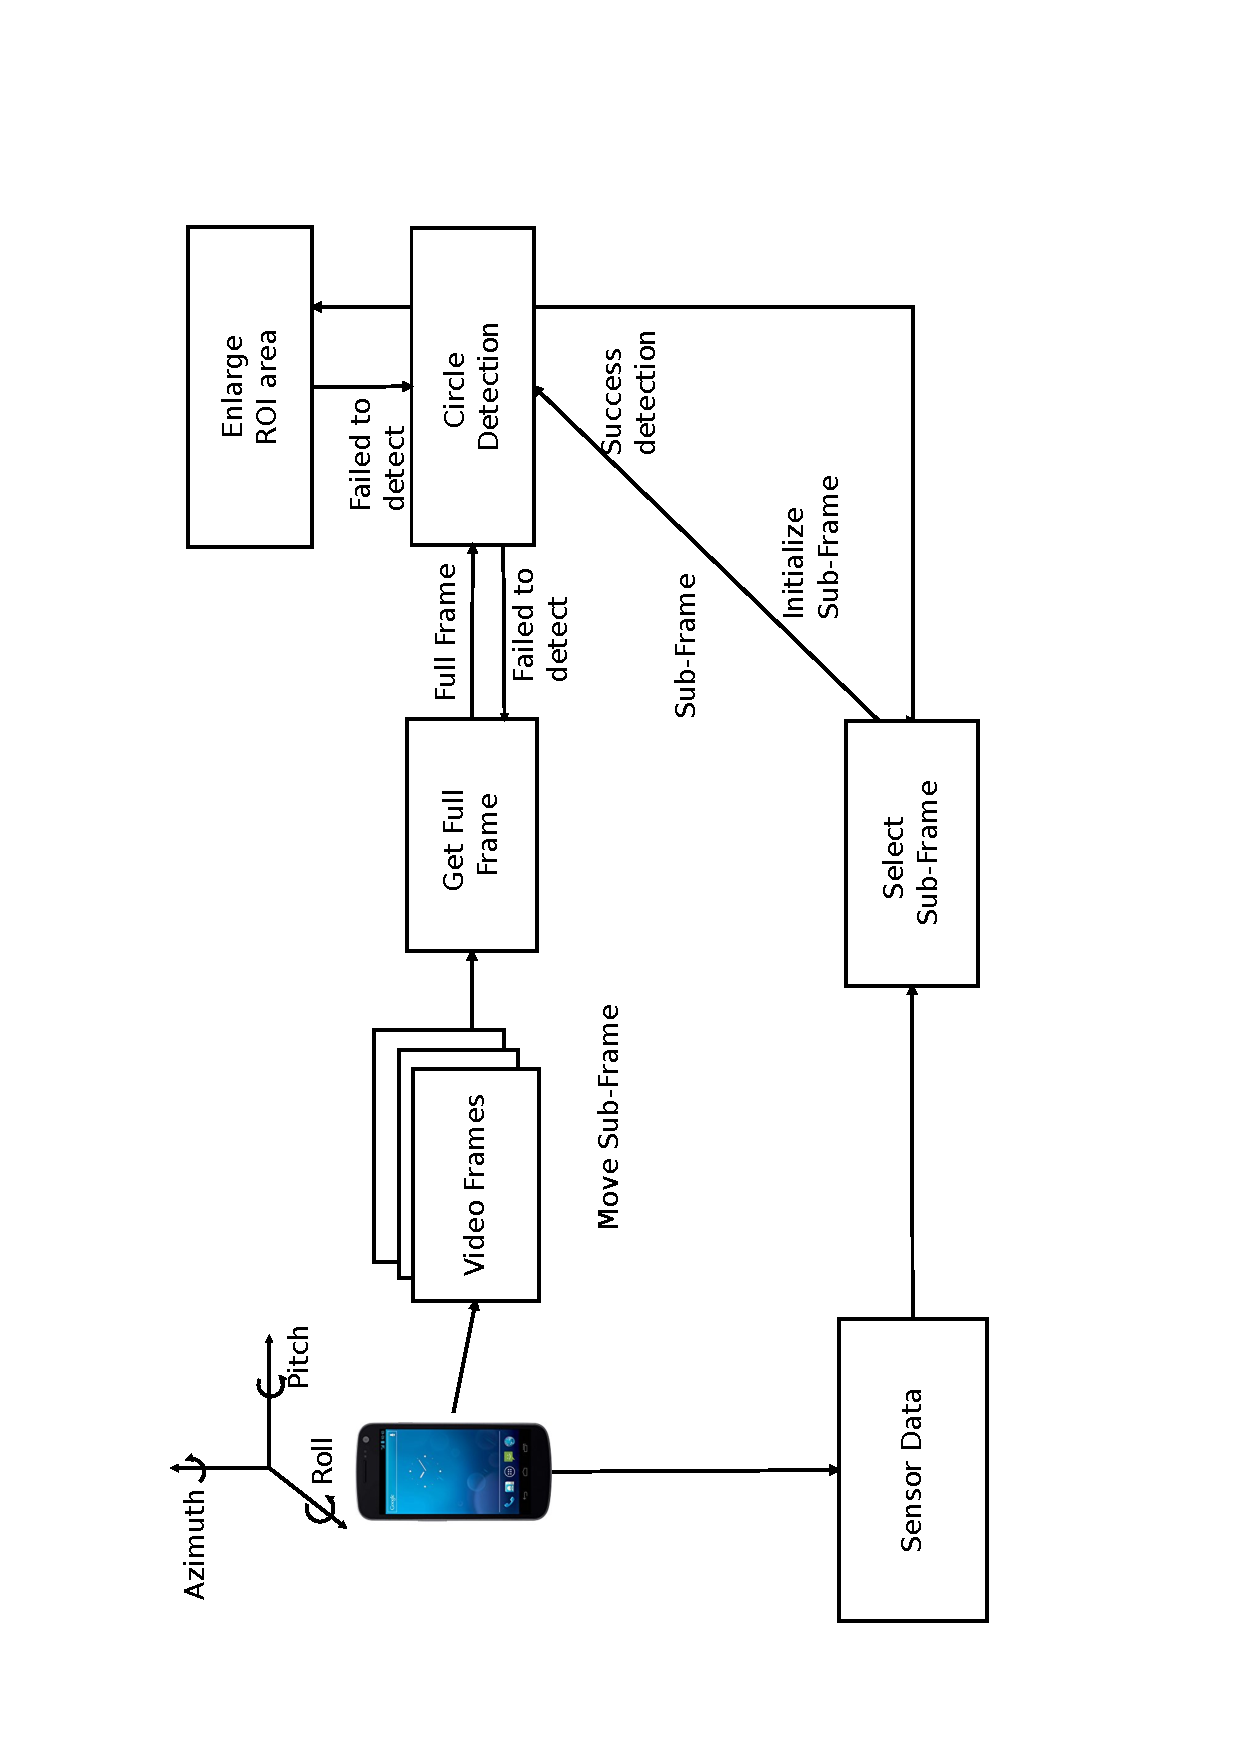
\includegraphics[width=5.2in]{figures/sysdia.pdf}
\caption{System Overview}
\label{f:sys_dia}
\end{figure}


Figure \ref{f:sys_dia} shows the overview of our system.
Using our smartphone app, we simultaneously record video and inertial sensor data.
Initially, we process the full region of the video frames to detect the traffic lights.
Once we successfully detect traffic lights in a video frame, we process only sub-parts of the subsequent frames using the sensor hints. 
For the subsequent frames, using the orientation change, we predict the region where the the traffic lights are likely to move and process only that region for detecting the traffic lights.
However, the prediction of region-of-interest (ROI) using the sensor hints can sometimes be incorrect.
In such cases, we gradually increase the area of the ROI until we detect traffic lights in that enlarged area. 
Note that the increment of the ROI can go up to the whole frame if there is no traffic lights in the frame or the traffic light detection algorithm fails to detect the existing traffic lights. 

The algorithm to detect traffic lights is same irrespective of processing of the full frame or a subpart of the frame.
Below, we discuss the the image processing algorithm for traffic light detection at first. 
Next, we discuss the procedure to select a subpart of a frame using sensor hints.


%We use three features of the traffic light, color, shape, and traffic bulb in a black box and the sensor feature of a smartphone as a system architecture for traffic light detection.
%% While recording the video we logged in the sensor data.
%% The first step of detection is the color filtering of the recorded videos.
%% Each video frames is consist of different colors.
%% In this step, each frame is filtered with only red and green pixel.
%% The traffic bulb shape is mostly circle.
%% To detect this characteristic we use Hough Circle  transformation\cite{hough_circle}.
%% Based on the traffic light detection position in video frames, we fix the region of interest area, which is a subpart of video frames.
%% After that, on next video frames the ROI change in respect to the sensor data. 


%% At first, we recorded videos along with the sensor data, gyroscope, accelerometer, pitch, roll, and azimuth.
%% These data have synchronization with our recorded video frames since we logged in sensor data while recording.
%% Now to detect the traffic light, we use three features of the traffic light.
%% Those are the color, shape of a traffic light and traffic light location in a black box.

\section{Image processing for traffic light detection}
The primary features of a traffic light is its bright red, yellow, or green color and the circular bulbs.
We use both these features for detecting the traffic lights. 
However, there can be other objects in the scene that can satisfy these properties such as circular red or green flower on people's clothing, red or green street signs etc.
To filter out such false detections, we use two heuristic filters, which utilize the fact that traffic lights are usually placed within a black box. 
Below, we discuss about these procedures in detail.

%% The first step of detection algorithm is color filtering of video frames.
%% Color filtering step filters out these candidate pixels from the video frames.


\subsection{Color space conversion}
The first step in our image processing pipeline is color space conversion.
We convert the BGR color space to HSV space.
To detect a specific color in BGR space, we need to use three different components (B, G, R).
However, HSV space has the property that we can detect a color based the single component, hue.
The range of hue values of each color are well defined and we utilze this range to keep the pixels of a desired color.


\subsection{Color filtering}
We only keep red and green pixels of a video frame for further processing in next stages.
In OpenCV \cite{opencv}, the hue range is from 0 to 180.
Table \ref{t:hue_range} shows the hue range for red and green colors.

\begin{table}[h!]
  \centering
  \caption{Hue range for red and green pixel.}
  \label{t:hue_range}
  \begin{tabular}{  l | c  }
    \hline
    Hue range for red & Lower 0 to 10 \\ \cline{2-2}
    & Upper 160 to 179 \\
    \hline \hline
    Hue range for green & 65 to 95 \\
    \hline
  \end{tabular}
\end{table}


\begin{figure*}[!ht]
\centering
\subfloat[Frame with red lights] {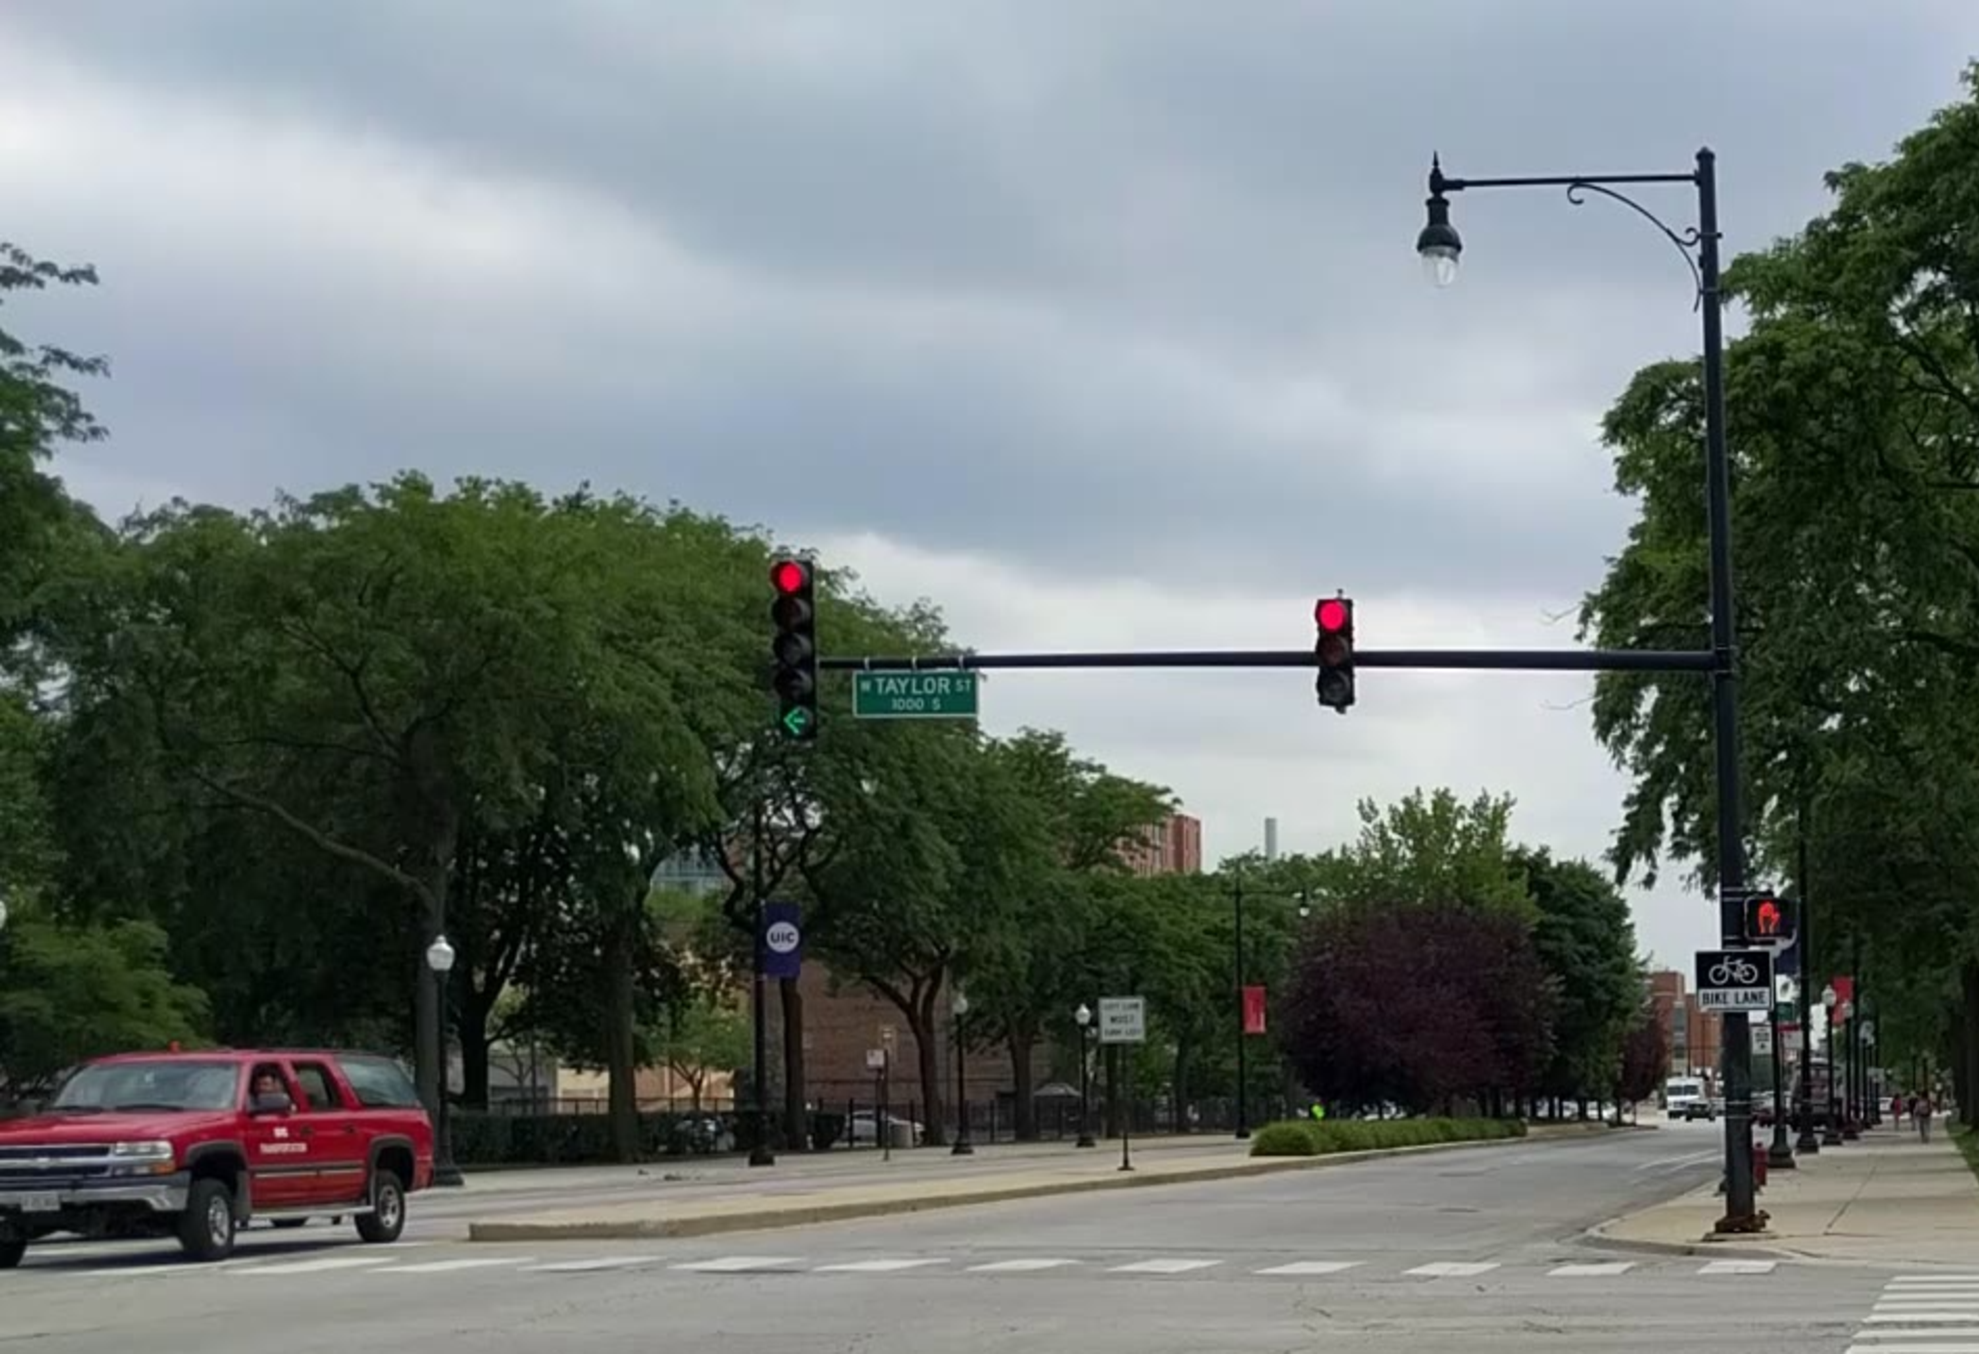
\includegraphics[width=3in]{images/frame301.pdf}}
\subfloat[Frame with green lights] {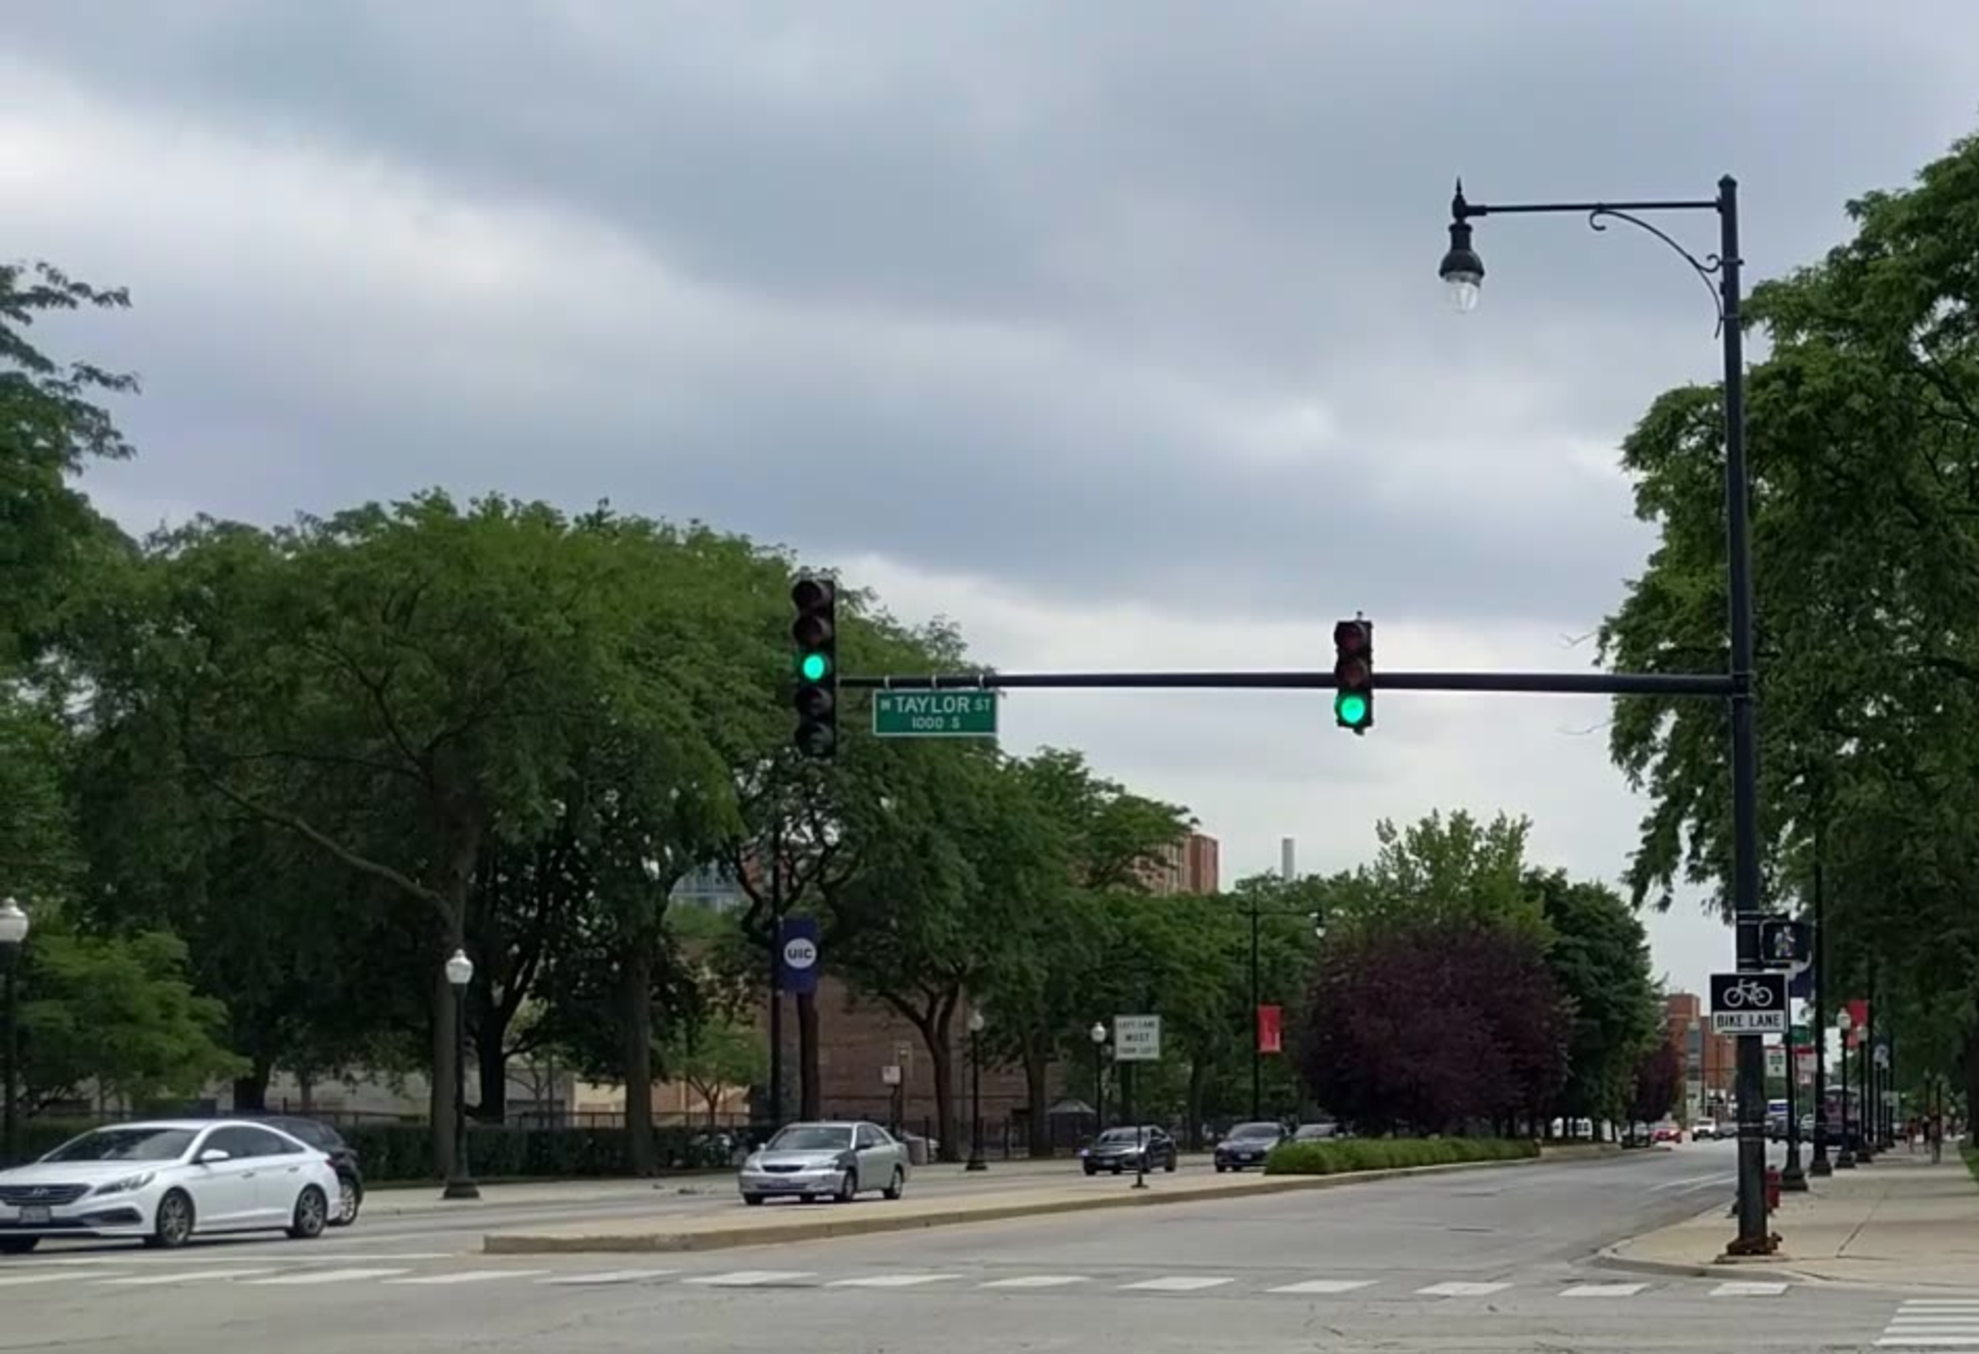
\includegraphics[width=3in]{images/frame502.pdf}}

\caption{Original videoframes.}
\label{f:org_img}
\end{figure*}

\begin{figure*}[!ht]
\centering
\subfloat[Frame with red lights] {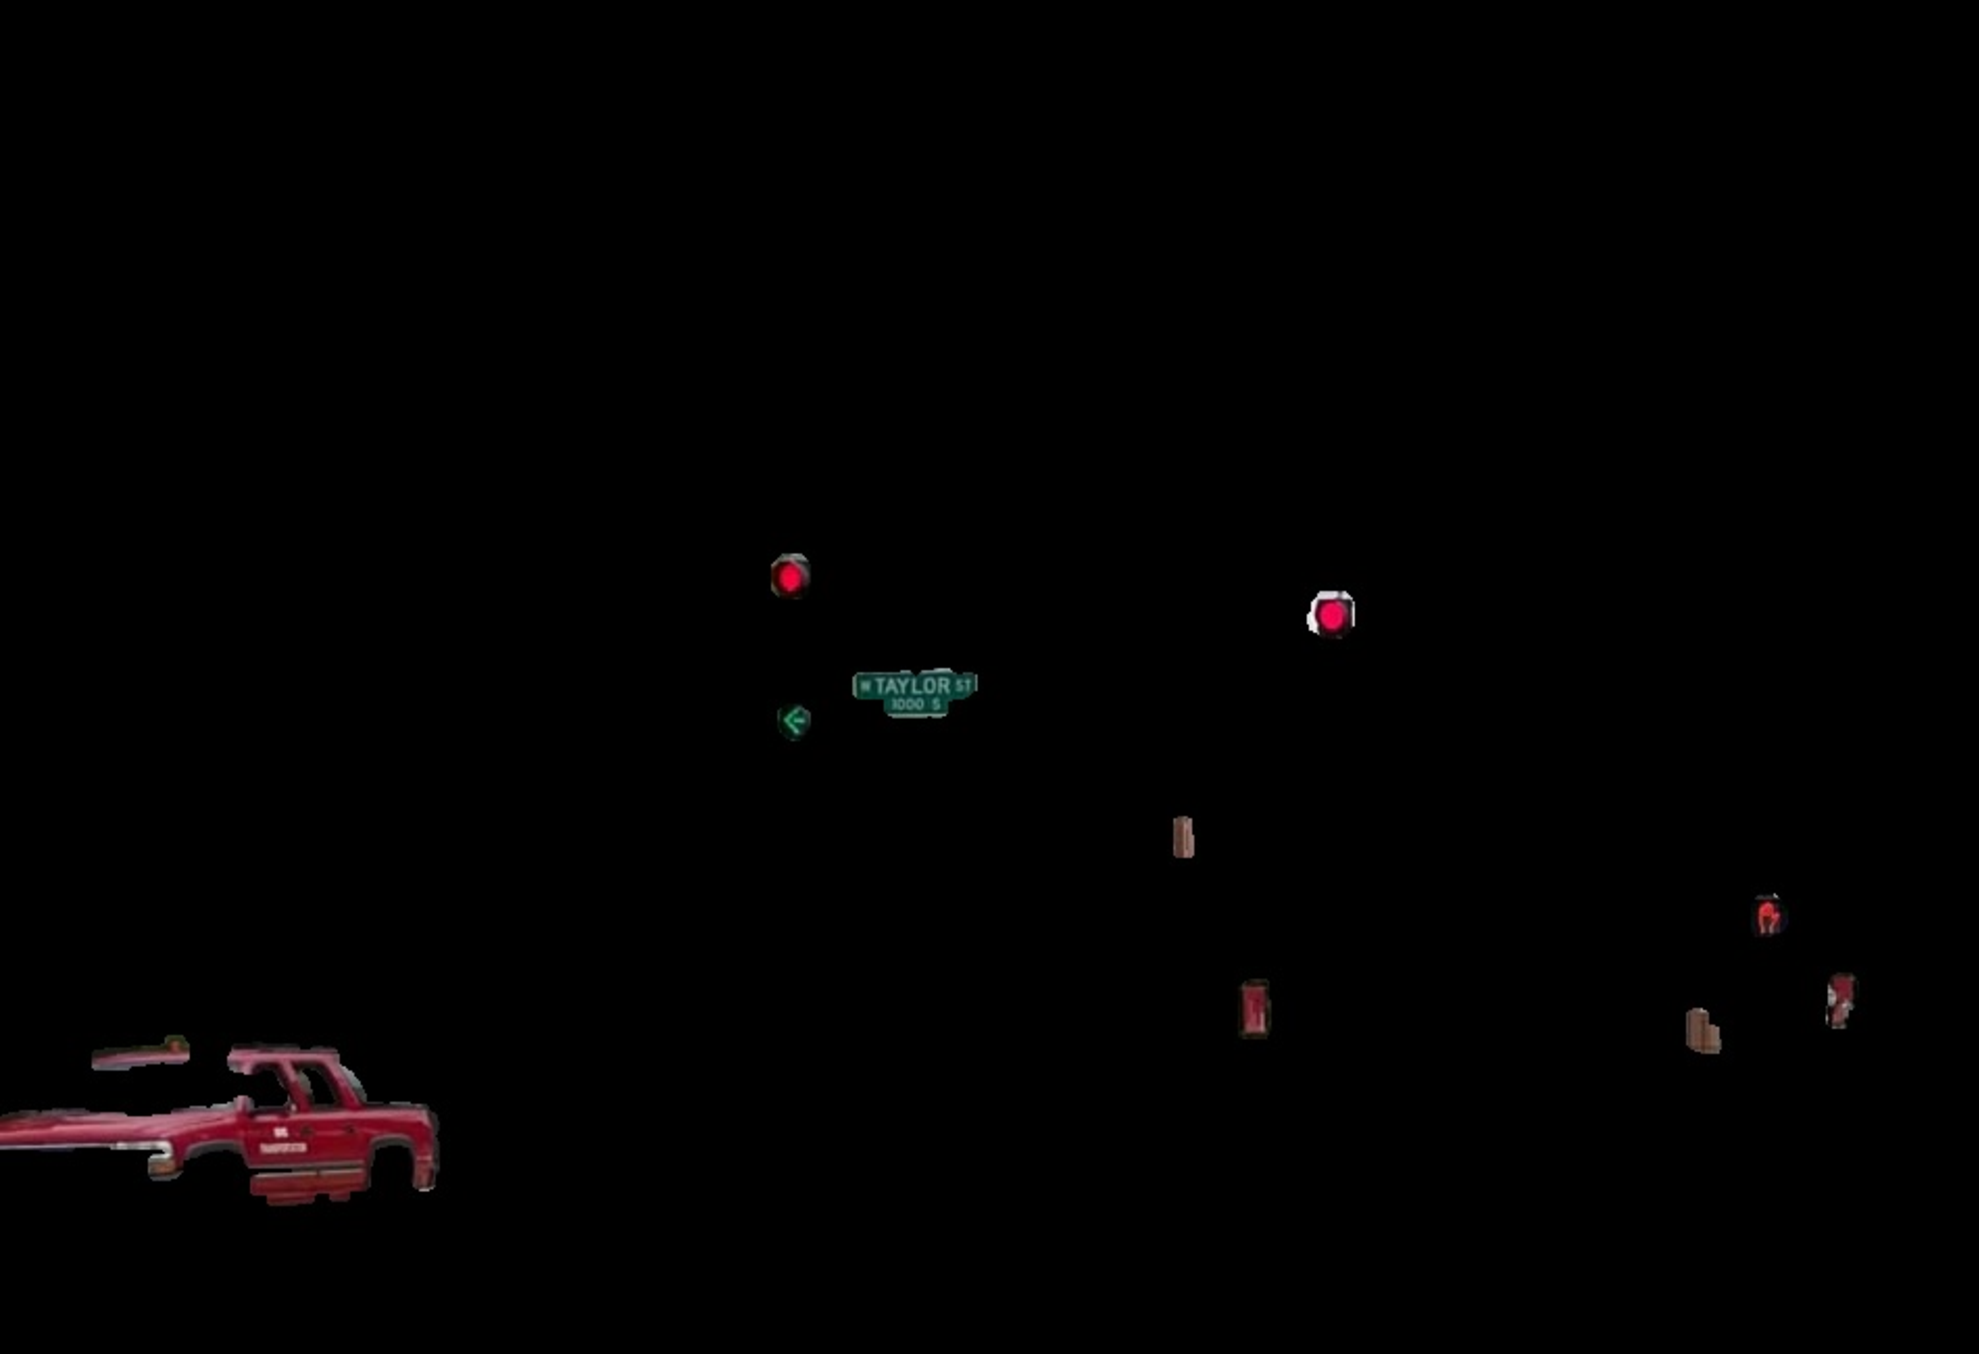
\includegraphics[width=3in]{images/RedGreenfiltering_red.pdf}}
\subfloat[Frame with green lights] {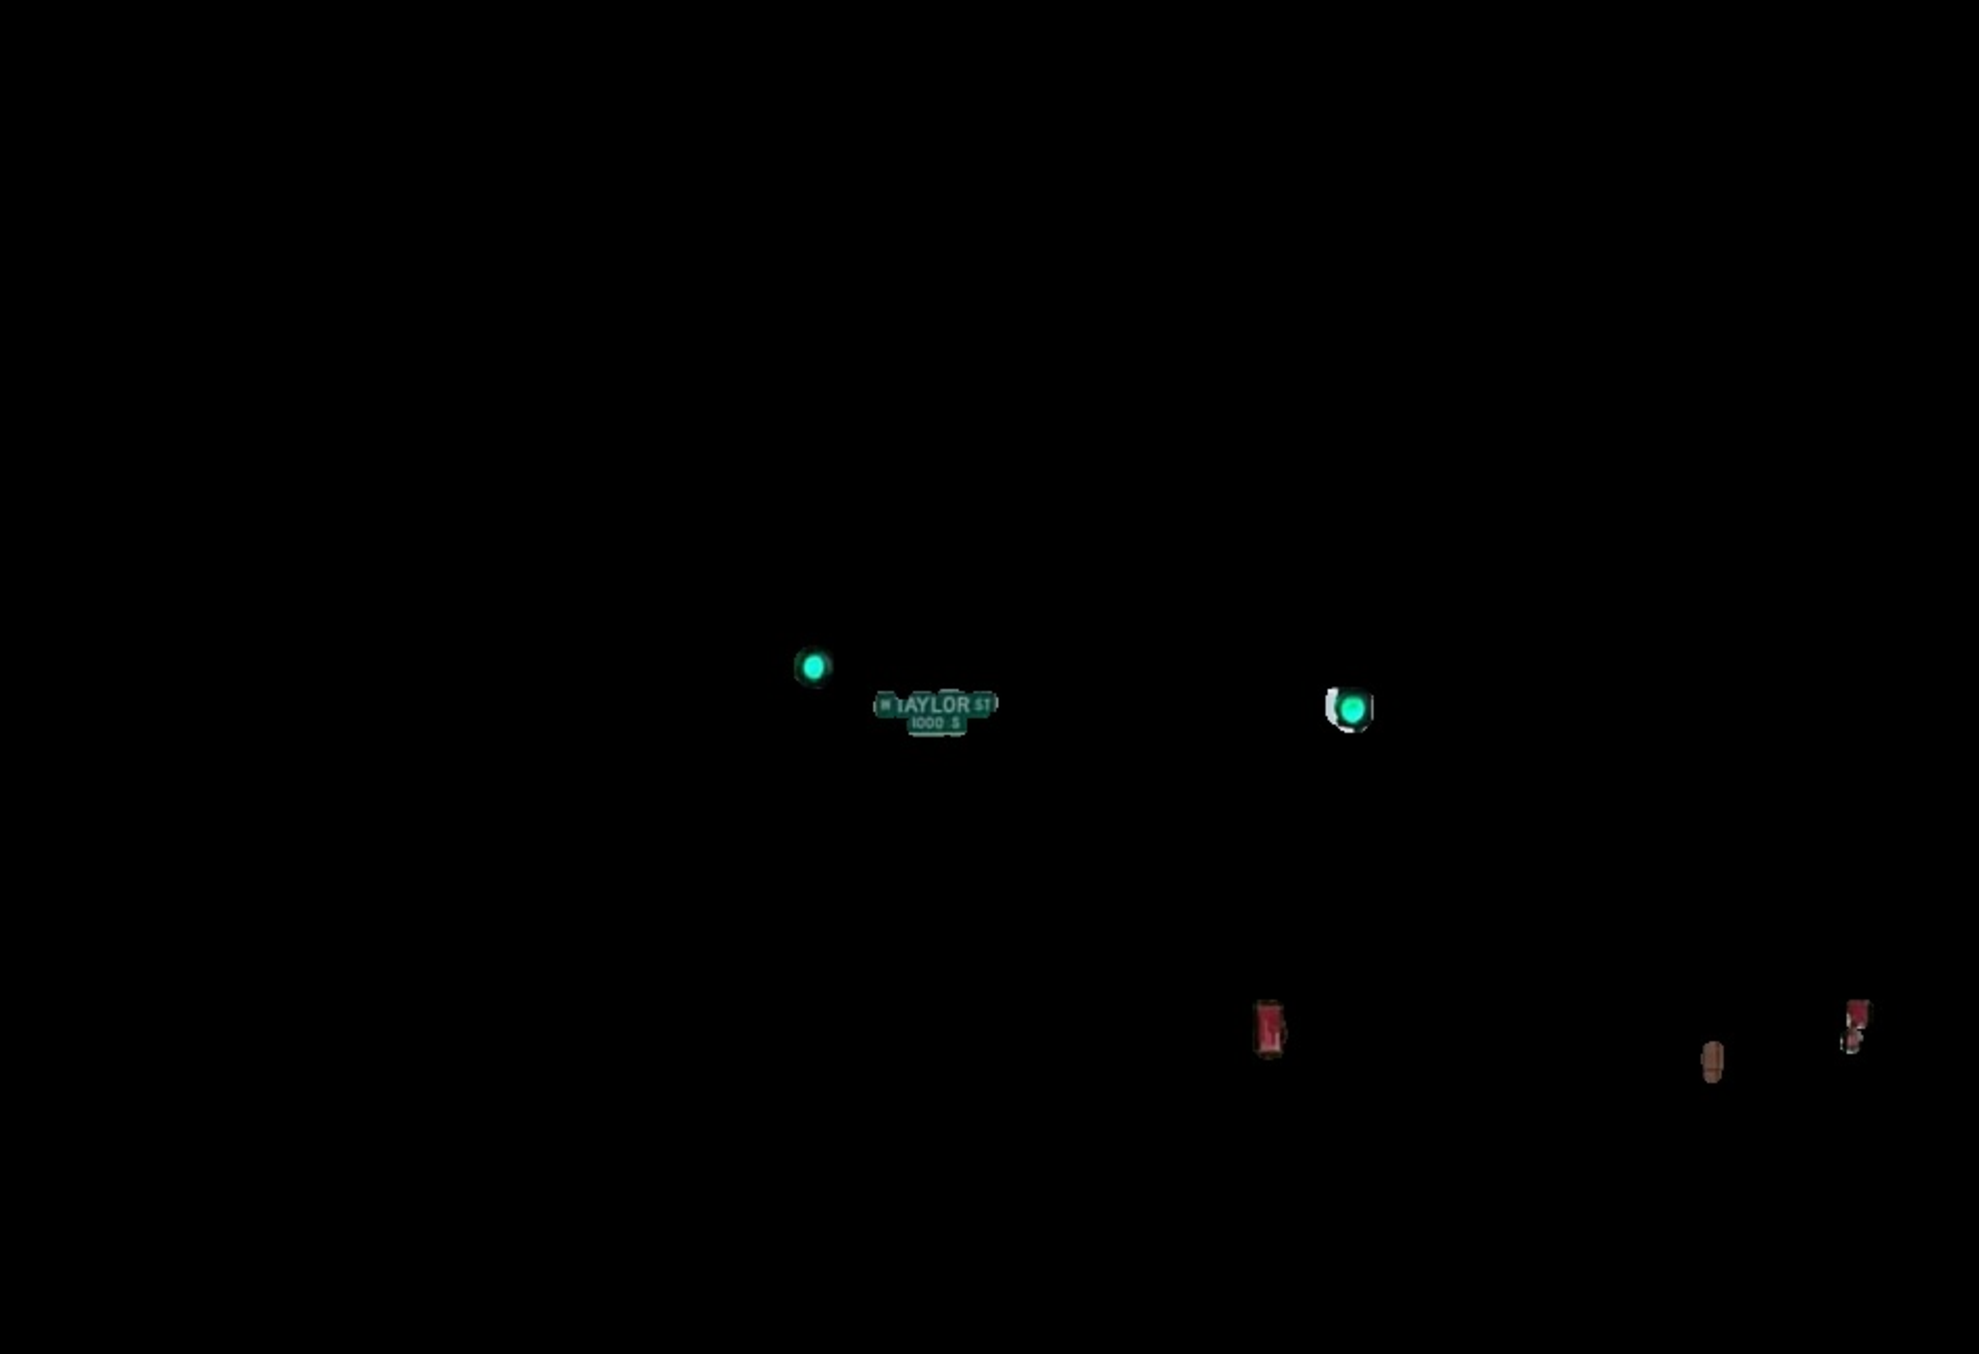
\includegraphics[width=3in]{images/RedGreenfiltering.pdf}}

\caption{Red green pixel filtering.}
\label{f:fil_img}
\end{figure*}

\ref{f:org_img}(a) shows the video frame with red traffic signal light and (b) shows the frame with green traffic signal light.
\ref{f:fil_img} shows the image with only red and green pixel.
(a) shows the filtering output with a red traffic light and (b) shows the filtering output with green traffic lights.
The color filtering process is computationally lightweight and it zeros out most of the pixels that reduce computational time to next steps.

\begin{figure}[h]
\centering
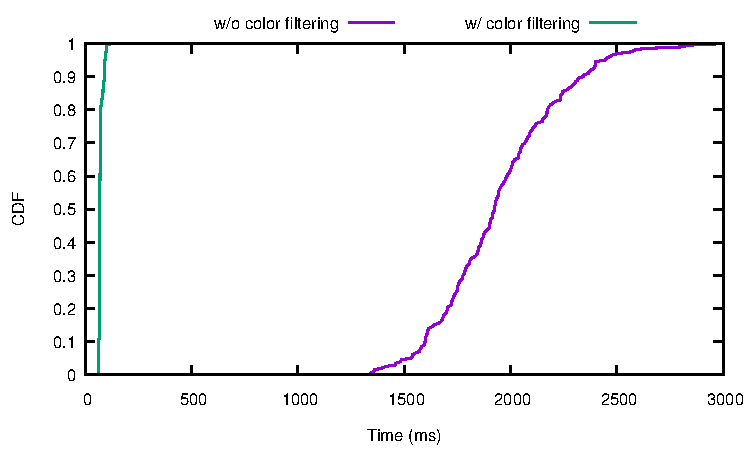
\includegraphics[width=5.2in]{plots/cdf_clrfil_full.pdf}
\caption{CDF for computational time comparison of the full videoframes with and without color filtering technique.}
\label{f:clrfil}
\end{figure}

\ref{f:clrfil} shows the computational time of the full videoframes with and without red and green color filtering technique.
It shows that color filtering process helps to reduce the processing time for all other steps significantly and this process itself is computationally lightweight.
\ref{f:clrfil} shows that the median of processing time is reducing from 2000 ms to 67 ms approximately. 

\subsection{Circularity check}
The next step of this detection algorithm is to detect the shape of traffic bulb (circle).
These filter images have only the desired pixel values.
To detect circle on this filtered images, we use Gaussian blur filter, in order to avoid false detection.
After this, we use the circle Hough Transform \cite{hough_circle} to detect the circles.
But, noise from the original images can fool the Hough transform to detect false and more circles.
As a solution to this problem, before converting our original BGR space frame to HSV space, a median filter is used.

\begin{figure*}[!ht]
\centering
\subfloat[Frame with red lights] {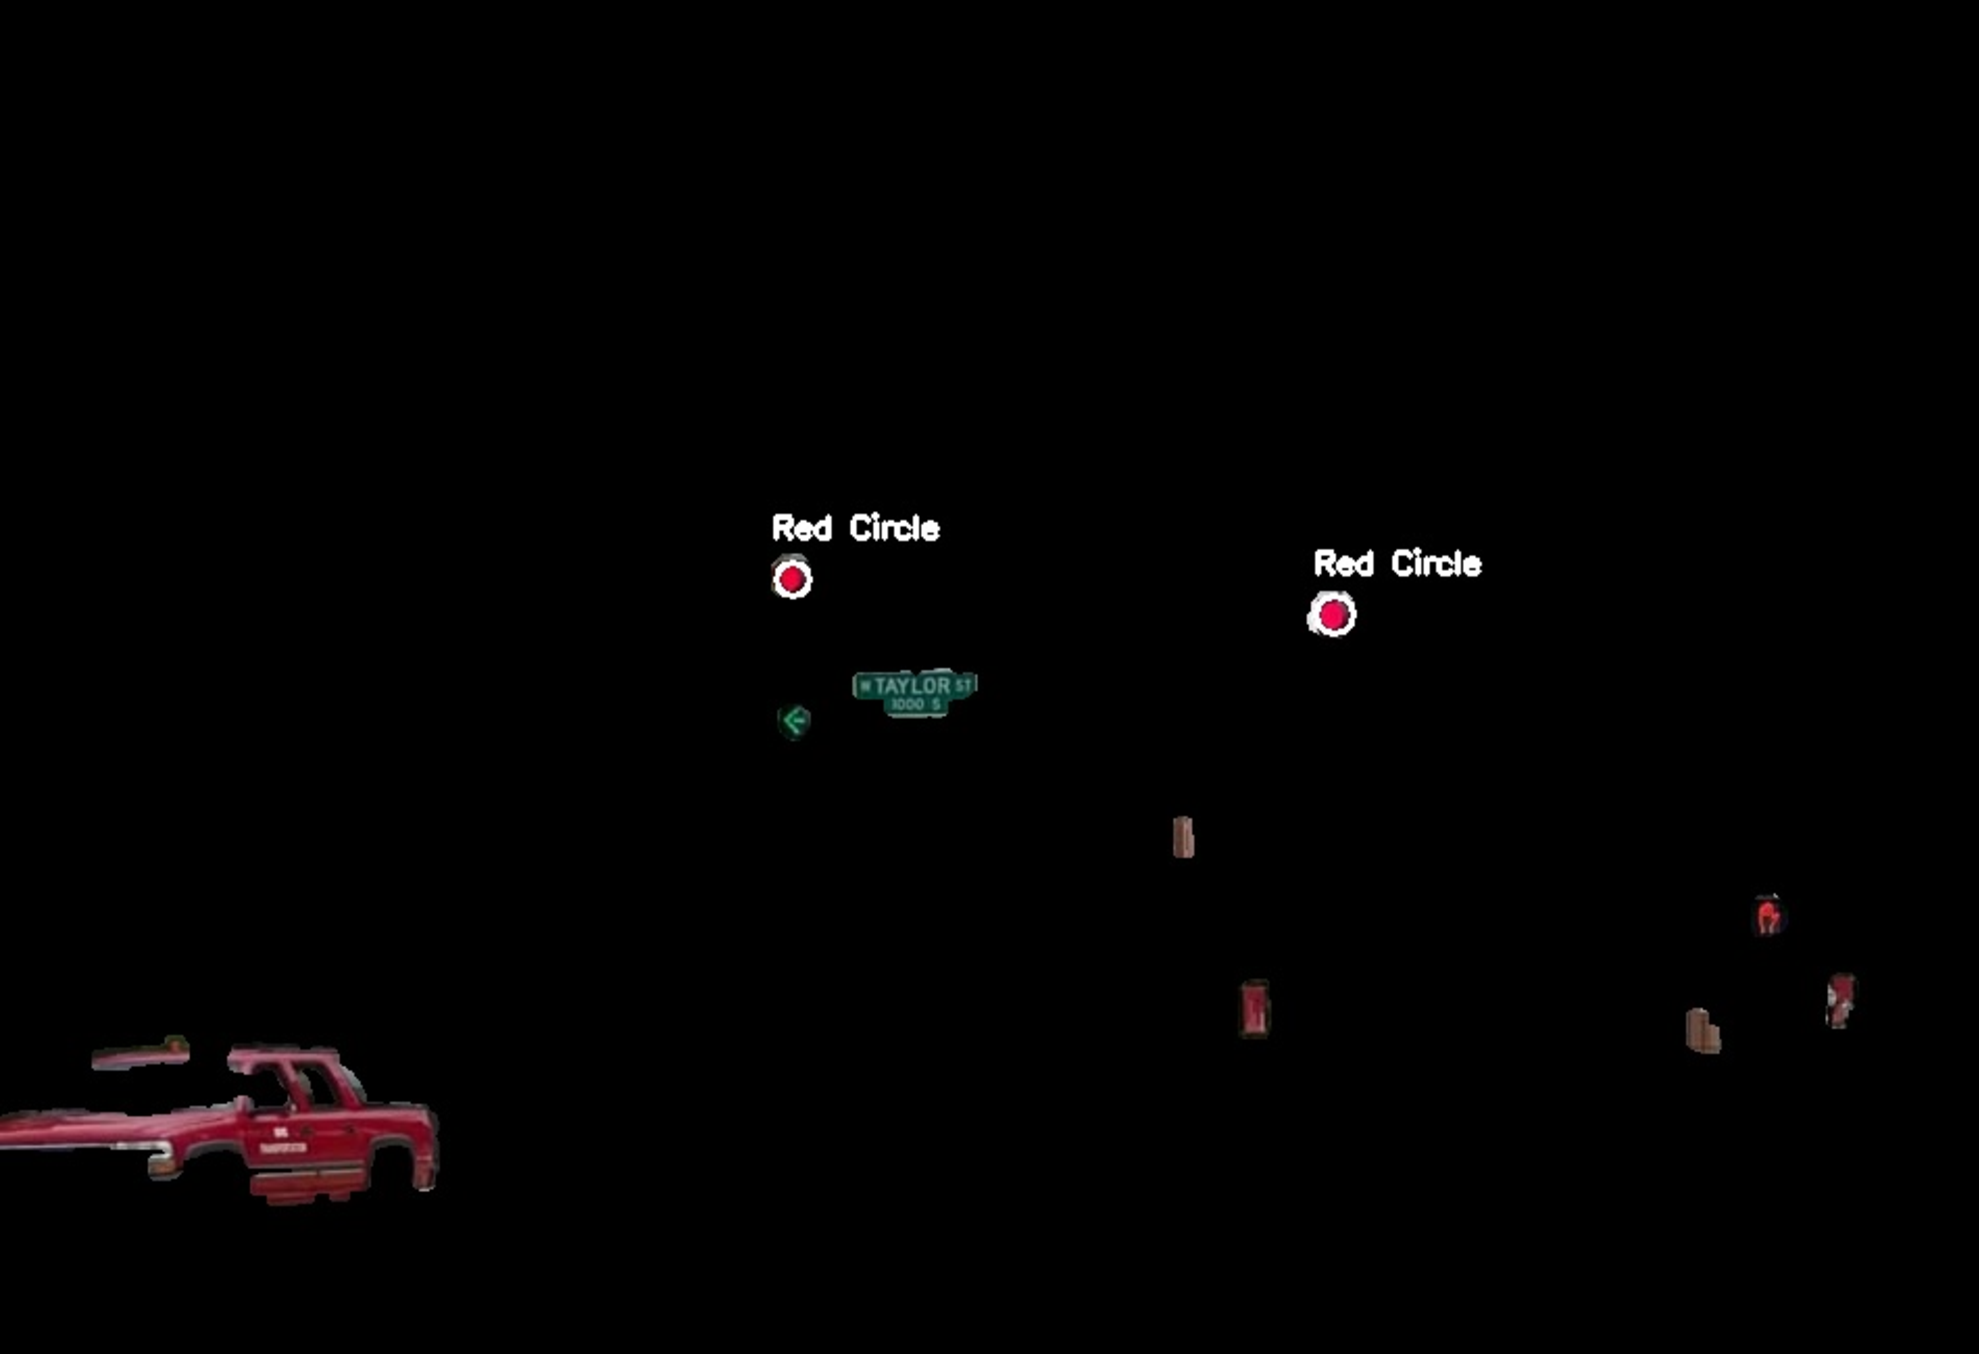
\includegraphics[width=3in]{images/Detectedredcircles.pdf}}
\subfloat[Frame with green lights] {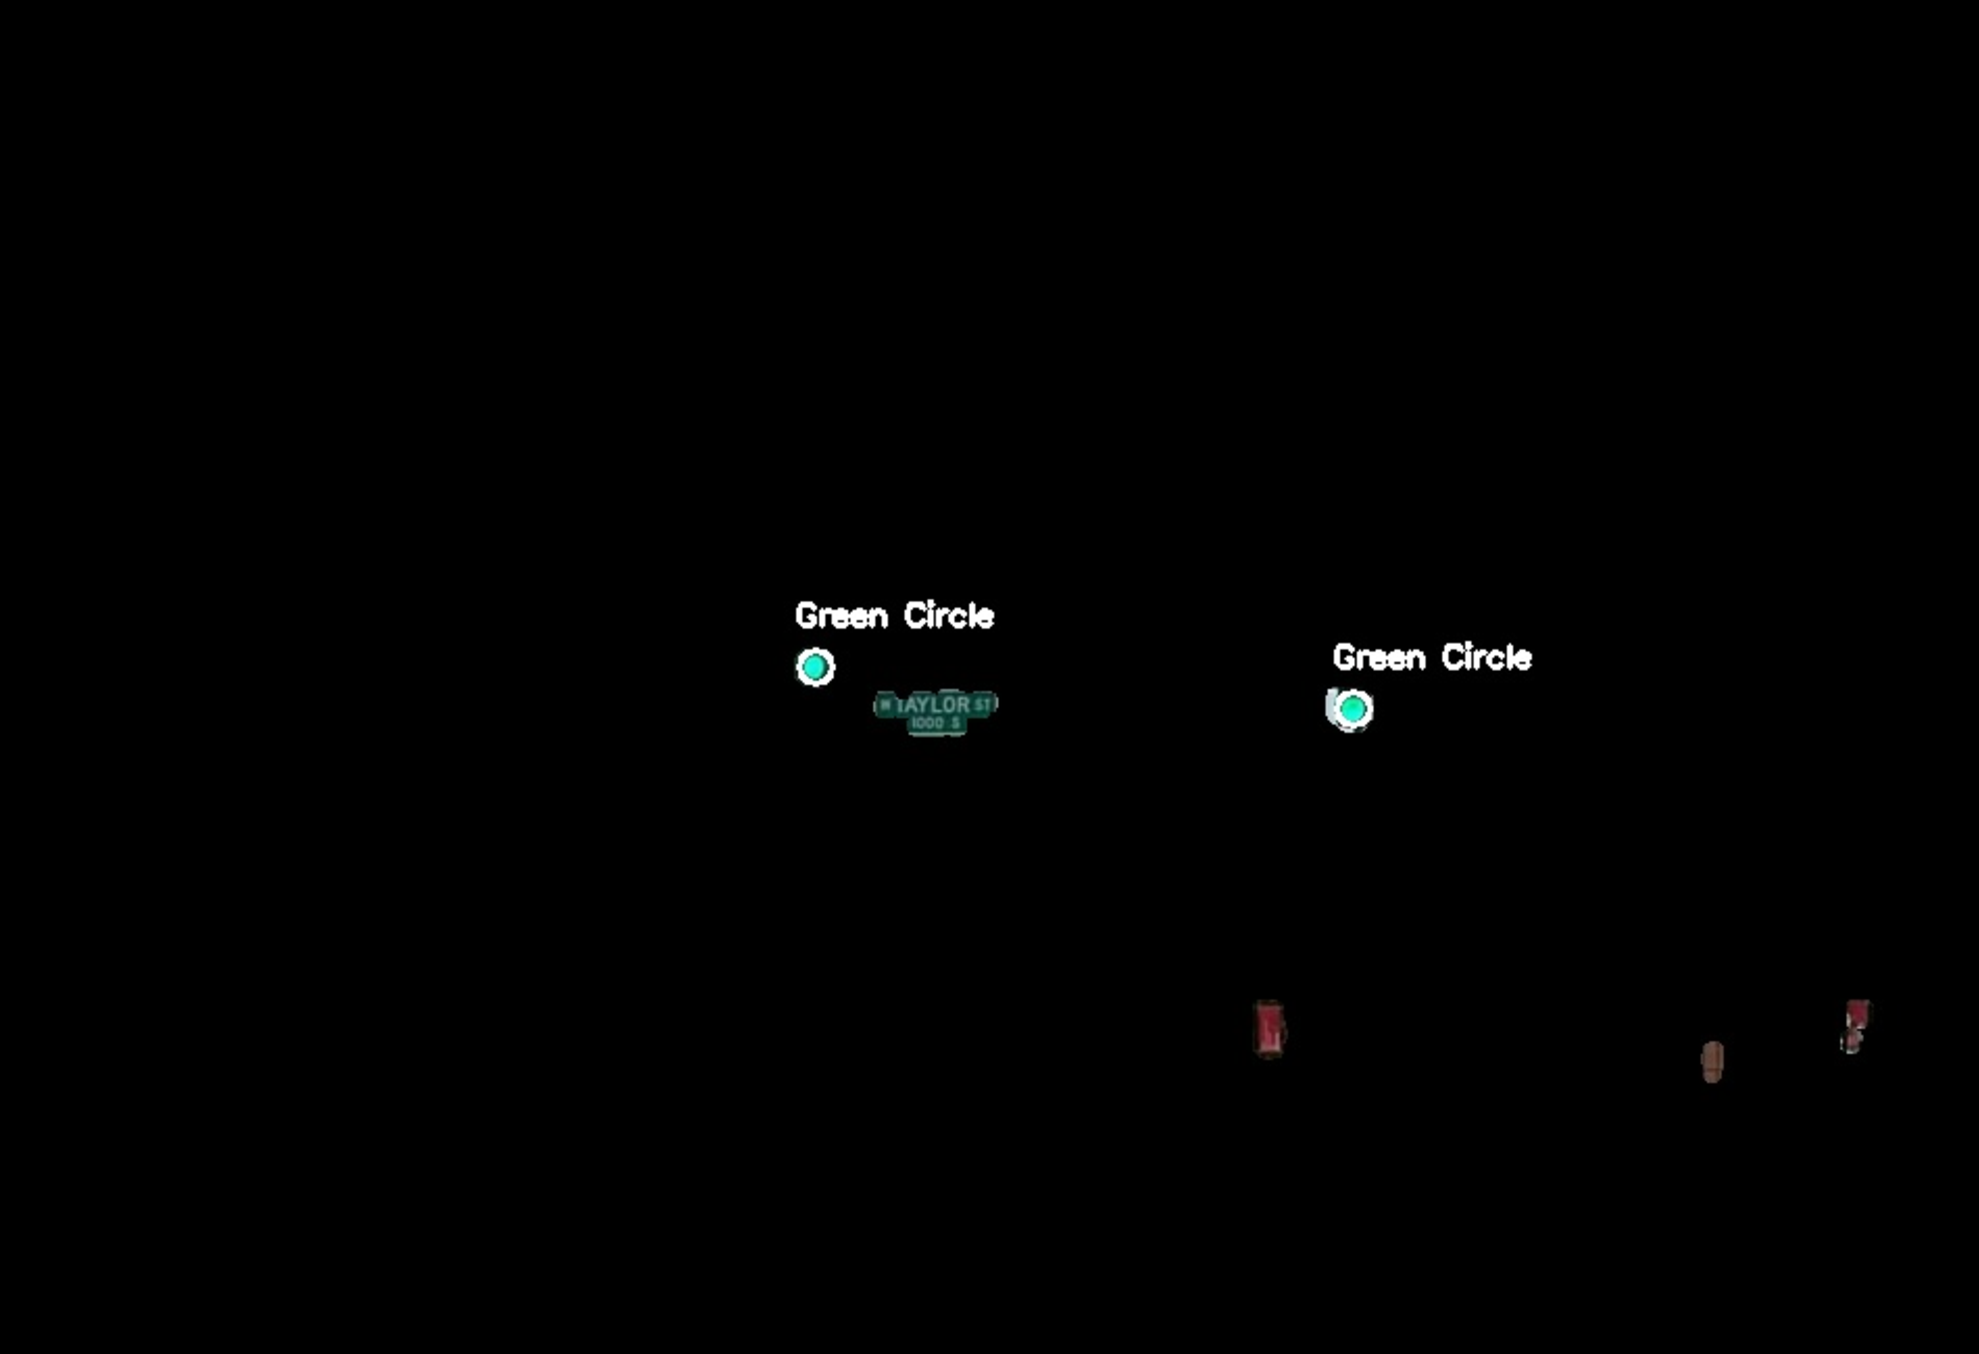
\includegraphics[width=3in]{images/Detectedgreencircles.pdf}}

\caption{Red green traffic bulb detection.}
\label{f:cir_img}
\end{figure*}

\ref{f:cir_img} shows the circle detection output.
(a) shows the red traffic light detection.
In this image, we have other red pixel values except for the traffic signal light.
But Hough circle transform can detect the circle precisely.
(b) shows the green traffic light detection output with Hough transform method.

\subsection{Heuristic filters}
\label{s:filter}
At this point, we have knowledge about the traffic bulb location and size (radius).
Now to detect if traffic bulb is in the black box, the other feature of our detection, we tried two heuristic filters.
Our first approach is to check pixels intensity of a circular area around the traffic bulb.
We use midpoint circle algorithm to find out the pixels value on a circular perimeter which is larger than our traffic bulb size.
our system gives a matrix with the count of pixels which has the intensity of a black color of all those points.
The intensity of black color can detect to check the Value of HSV space.
For black color, the range of the Value is very low, less than 40-45.
If this count is greater than our threshold we select that circle as our traffic bulb.
But we face some false detection problem with this approach.
Since the intensity of traffic bulb color is high and it spreads out also.
So we can not get a successful result with this approach.

\begin{figure*}[ht]
\centering
\subfloat[Red traffic bulb] {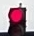
\includegraphics[width=2.2in]{images/redlight.jpg}}
\hfill
\subfloat[Green traffic bulb] {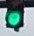
\includegraphics[width=2.2in]{images/greenlight.jpg}}\\

\caption{Red and green traffic bulb intensity.}
\label{f:bulb_int}
\end{figure*}

\ref{f:bulb_int} shows the red and green traffic bulb intensity.
We can see that the color spreads out around the exact circle area.
So the black color intensity measurement around the bulb circle area using midpoint circle algorithm is not giving an actual result.

Our second approach is to scan a rectangle frame  around the traffic light.
Traffic bulbs locate in a black box, which can place in horizontally or vertically in street.
To make our approach more global we scan all around the traffic light to check the intensity.
Our system gives a matrix of the no of pixels that have the intensity same as black color.
If this pixel no is more than our threshold value we consider that the detected circle is in the traffic signal black box and we finally detect that circle as our traffic bulb.
\begin{figure}[!ht]
\centering
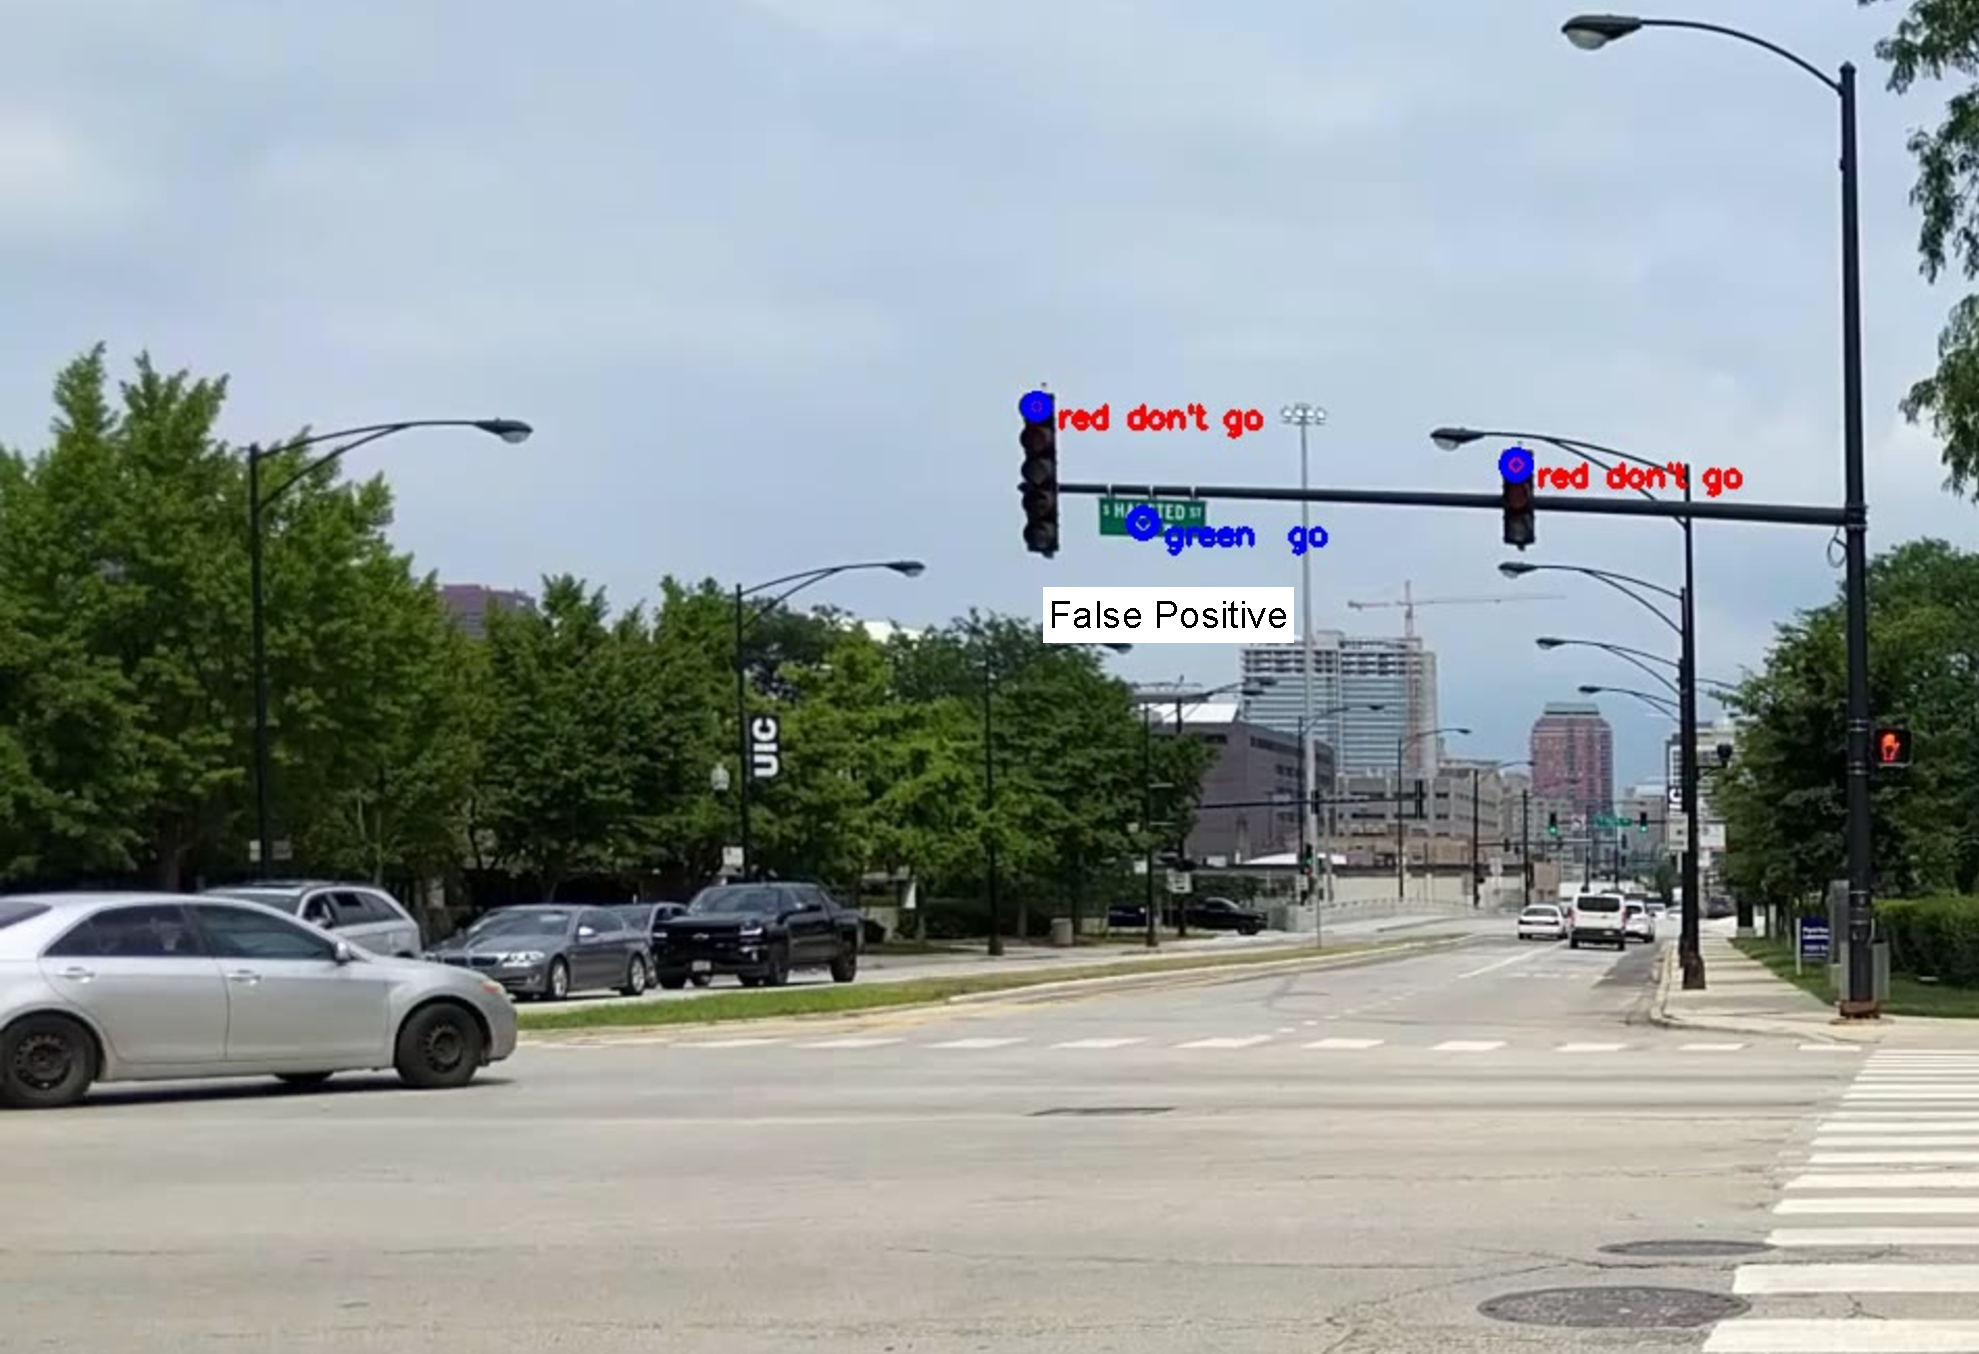
\includegraphics[width=4.2in]{images/norec_filter.pdf}
\caption{Output not using black box checking filter.}
\label{f:norec_filter}
\end{figure}

\ref{f:norec_filter} shows there is one green false positive between two red traffic light.
That false green circle actually a street nameplate and around that there is no black box.
So when we use our black box checking filter we can remove this false positive detection.
\ref{f:rec_filter} shows the output after using our heuristic black box checking filter.




\begin{figure}[ht!]
\centering
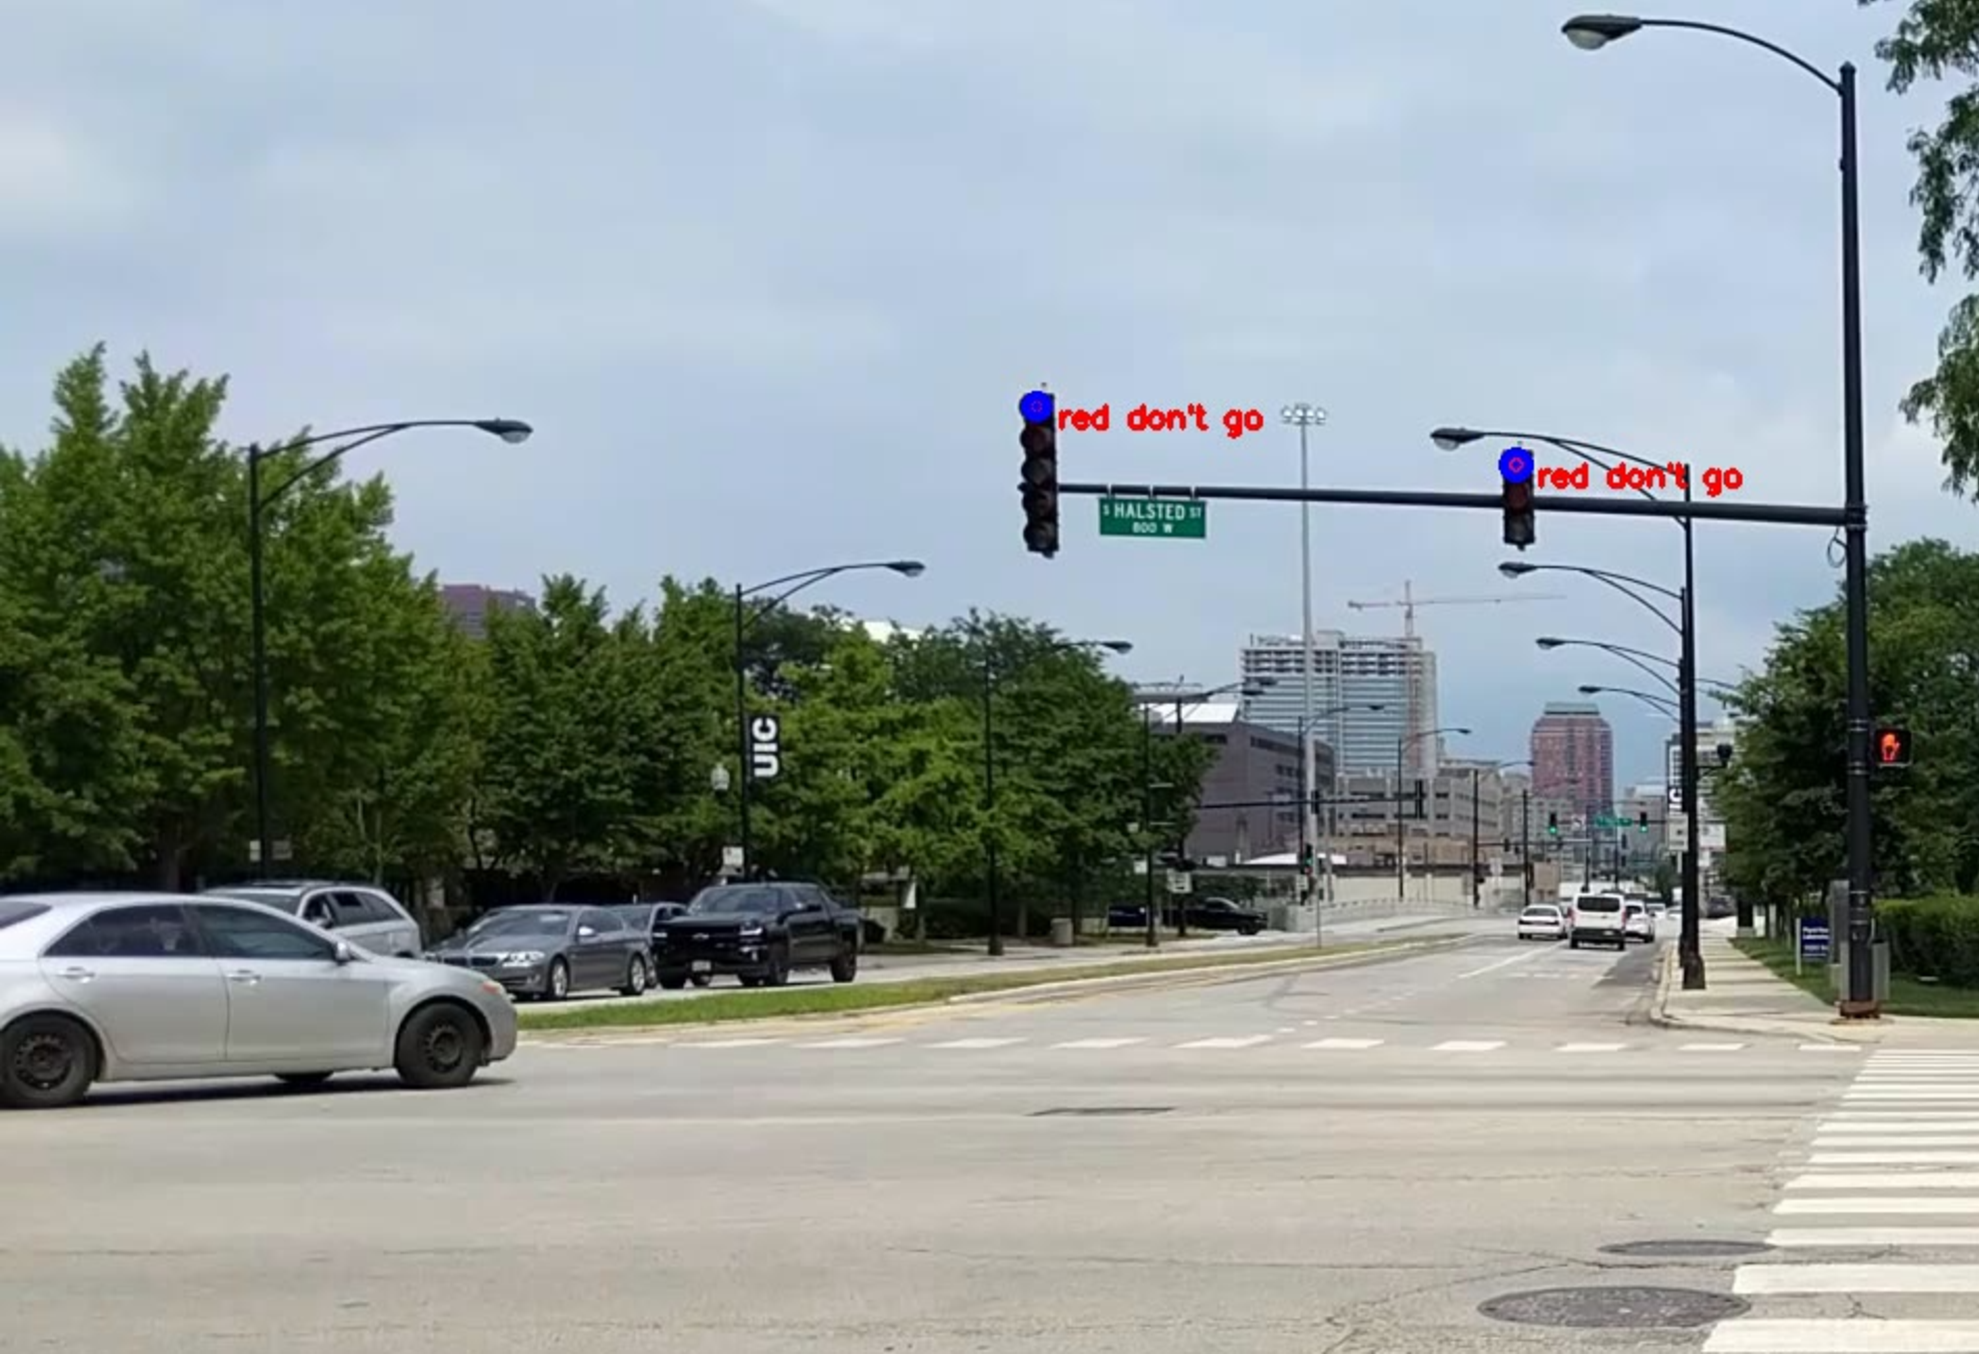
\includegraphics[width=4.2in]{images/rec_filter.pdf}
\caption{Output using black box checking filter.}
\label{f:rec_filter}
\end{figure}

\section{Sensor fusion for subpart selection}

\subsection{Synchronization of sensors and video frames}
To improve our detection we also use the smartphone's sensor data hints.
Our system logged the sensor data while recording the video.
From the logged data we know the time for sensor data registered.
We have the time when the video is recorded.
After that, we synchronized our data with the video using the starting time of the video and the frame rate.
So, using the frame rate and starting time we know the time for each frame, and from the logged sensor data, we know the sensor value corresponds to the time.
Using this time and our frame time we interpolated sensor hints if we miss any data corresponding to that frame.
Finally, we get the synchronized sensor data with our recorded video.

\ref{} shows the interface of our android app.
So when we start recording the pitch, roll and azimuth display in the screen and also start registering in a file.

\subsection{Region-Of-Interest selection}
\label{s:roi}
Now, when we detect a traffic light in our video frame successfully using the color, shape of the traffic light and the characteristics of traffic bulb being in a box, we have the idea of the position of the traffic light.
With this idea we subdivide our video frame making a region of interest area.
When we move to the next frame, we have a prior knowledge of traffic light position and we know the sensor data, pitch, roll, and azimuth of this frame.
Using these sensor data of the current frame and the previous frame we have the idea of the movement of the traffic light.
With this change of movement, the ROI also moves to the direction of change.
\ref{f:rec_mv}shows the movement of ROI with the change of pitch and azimuth of our recorded video.
Apart from this, when our system can not detect any circle in our specific ROI area, it updates the ROI and tries to detect the light.

\begin{figure*}[!ht]
\centering
\subfloat[Initial ROI] {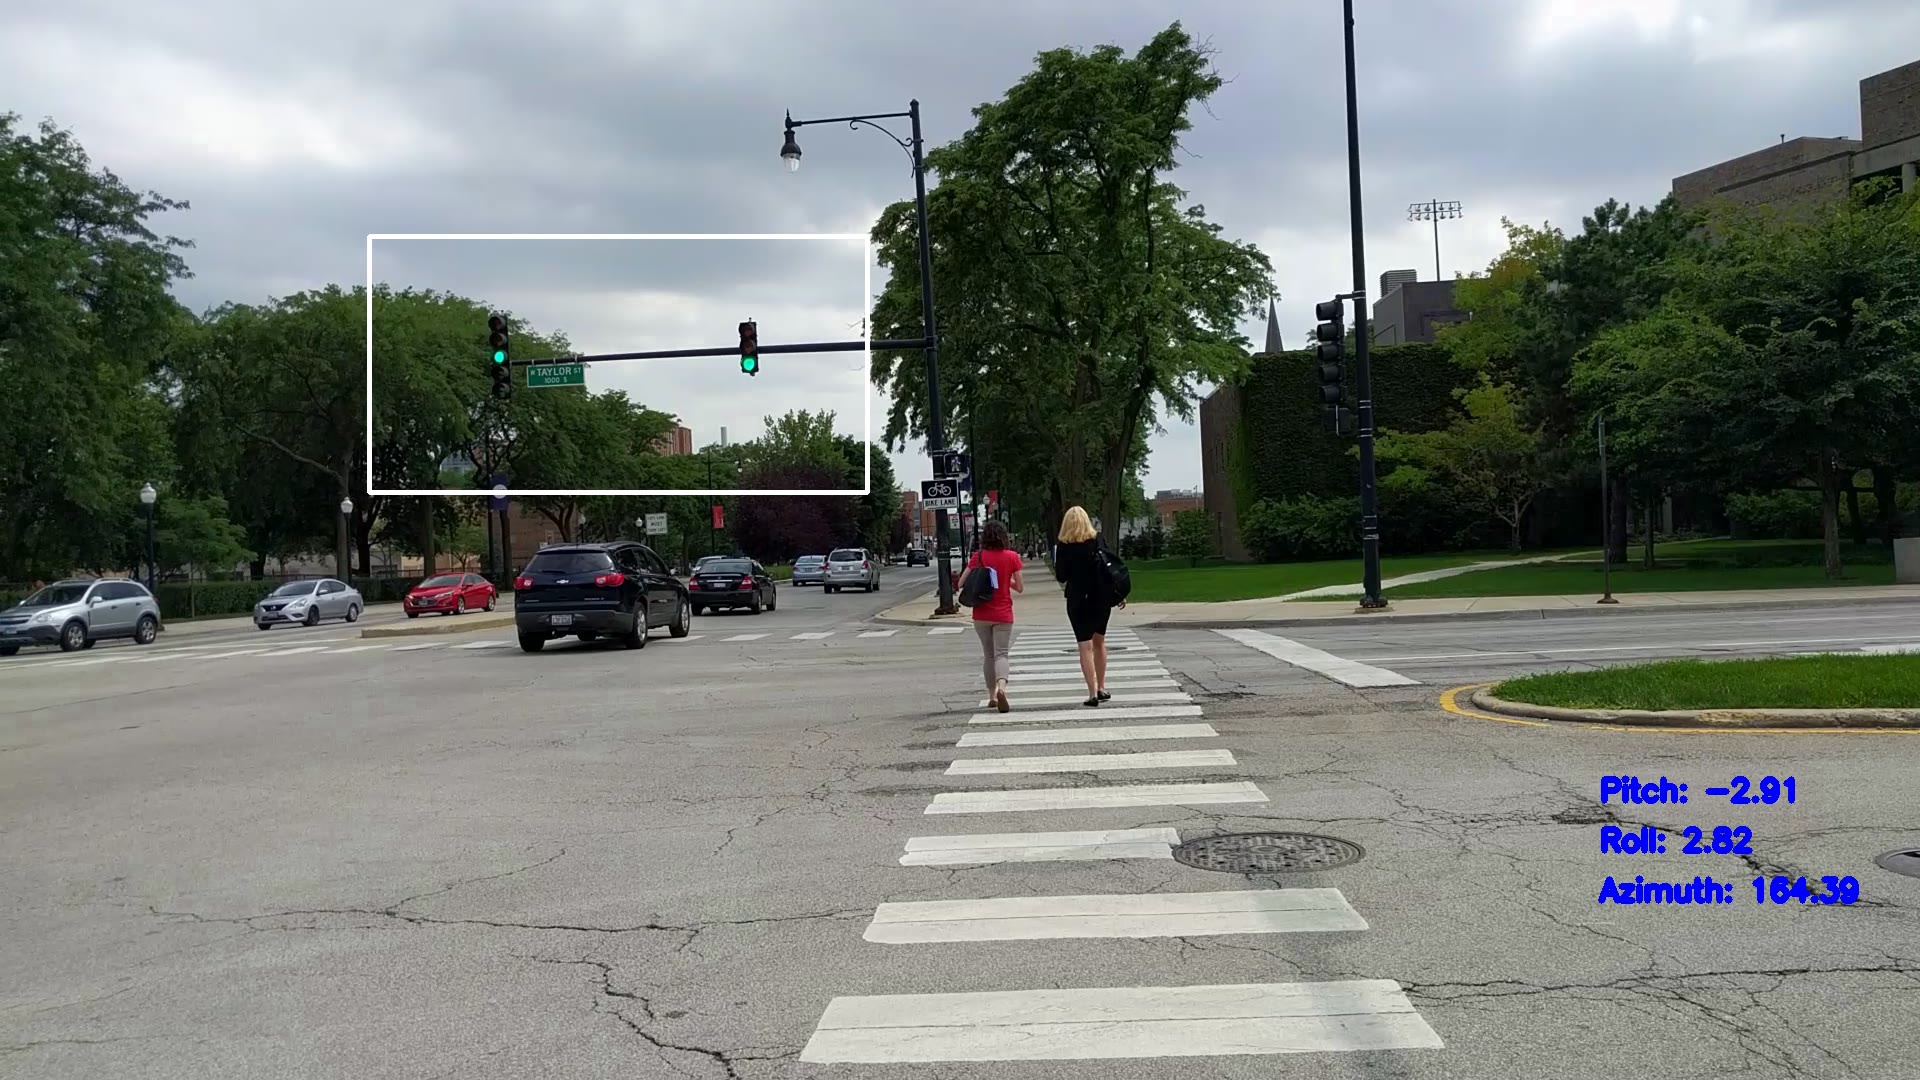
\includegraphics[width=4.2in]{images/rec_mv.jpg}}\\
\subfloat[Movement with change of sensor data] {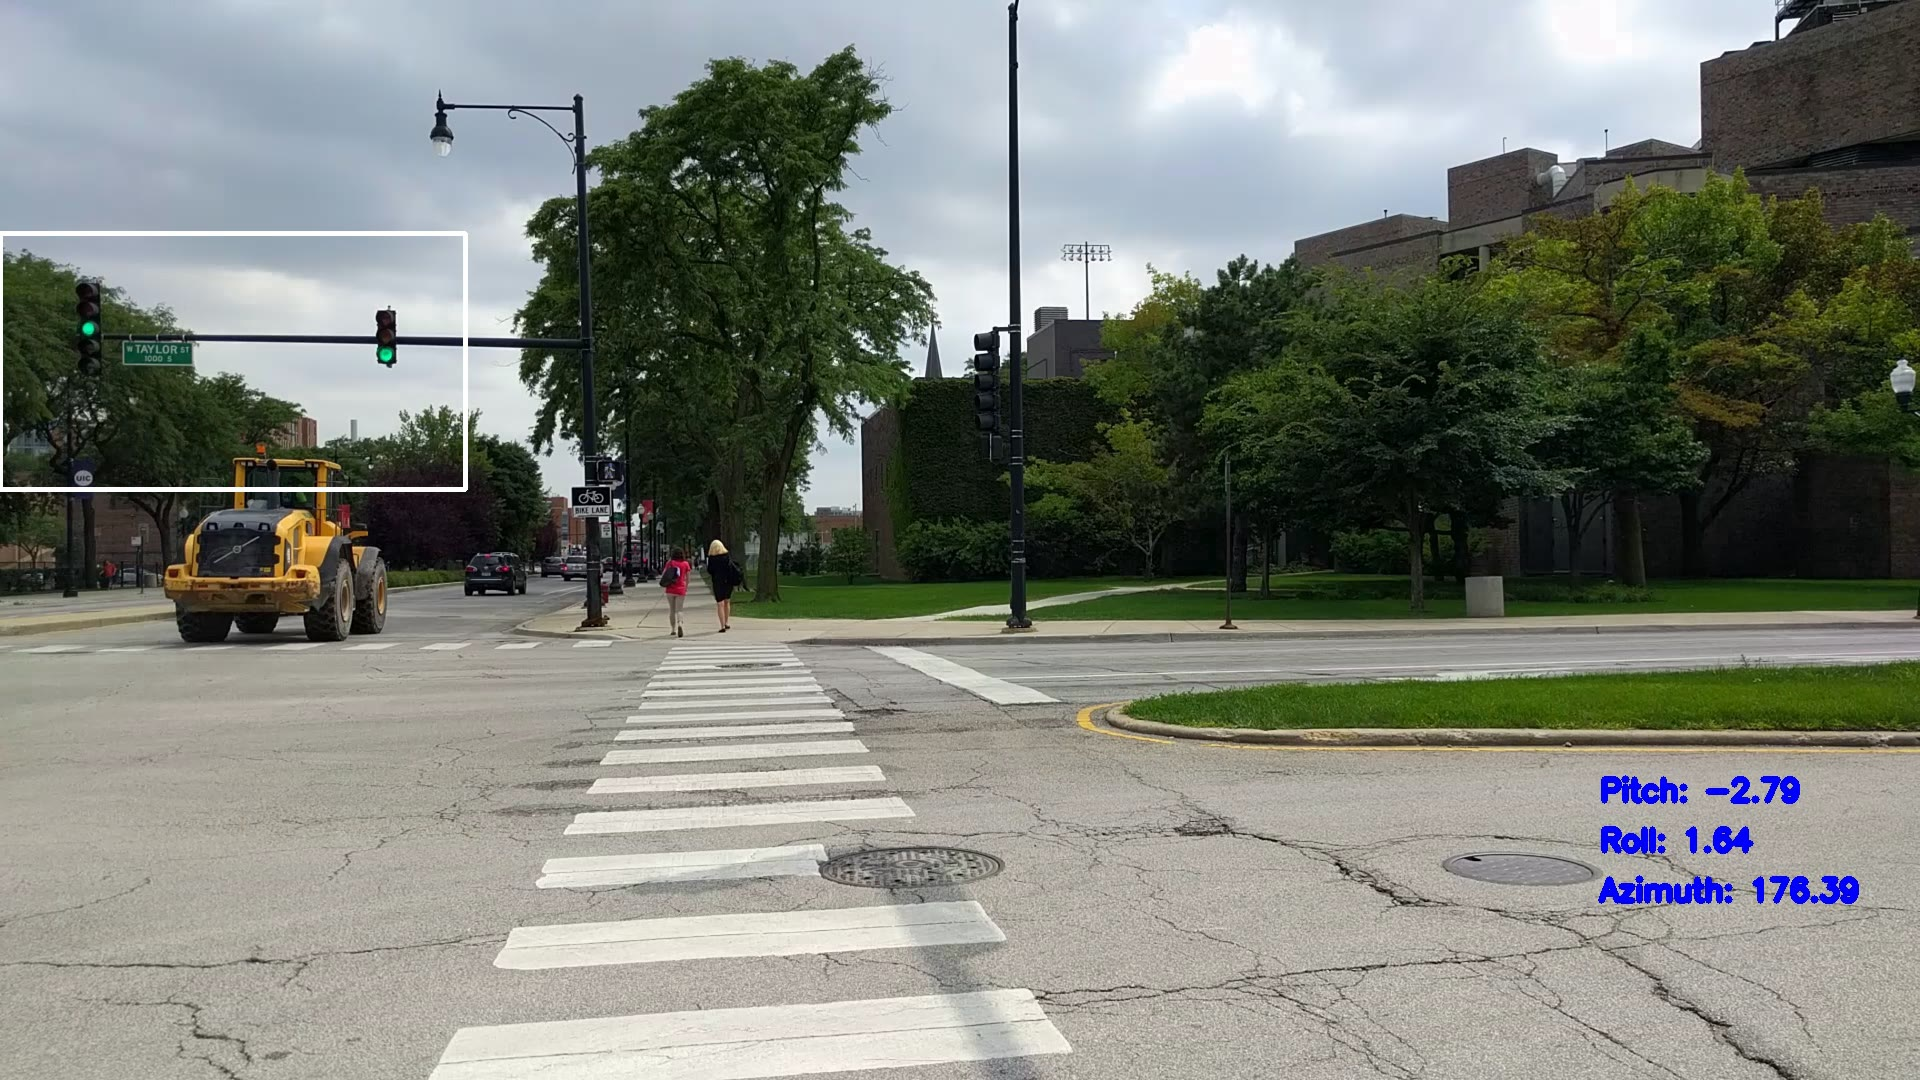
\includegraphics[width=4.2in]{images/rec_mv1.jpg}}\\
\subfloat[Movement with change of sensor data] {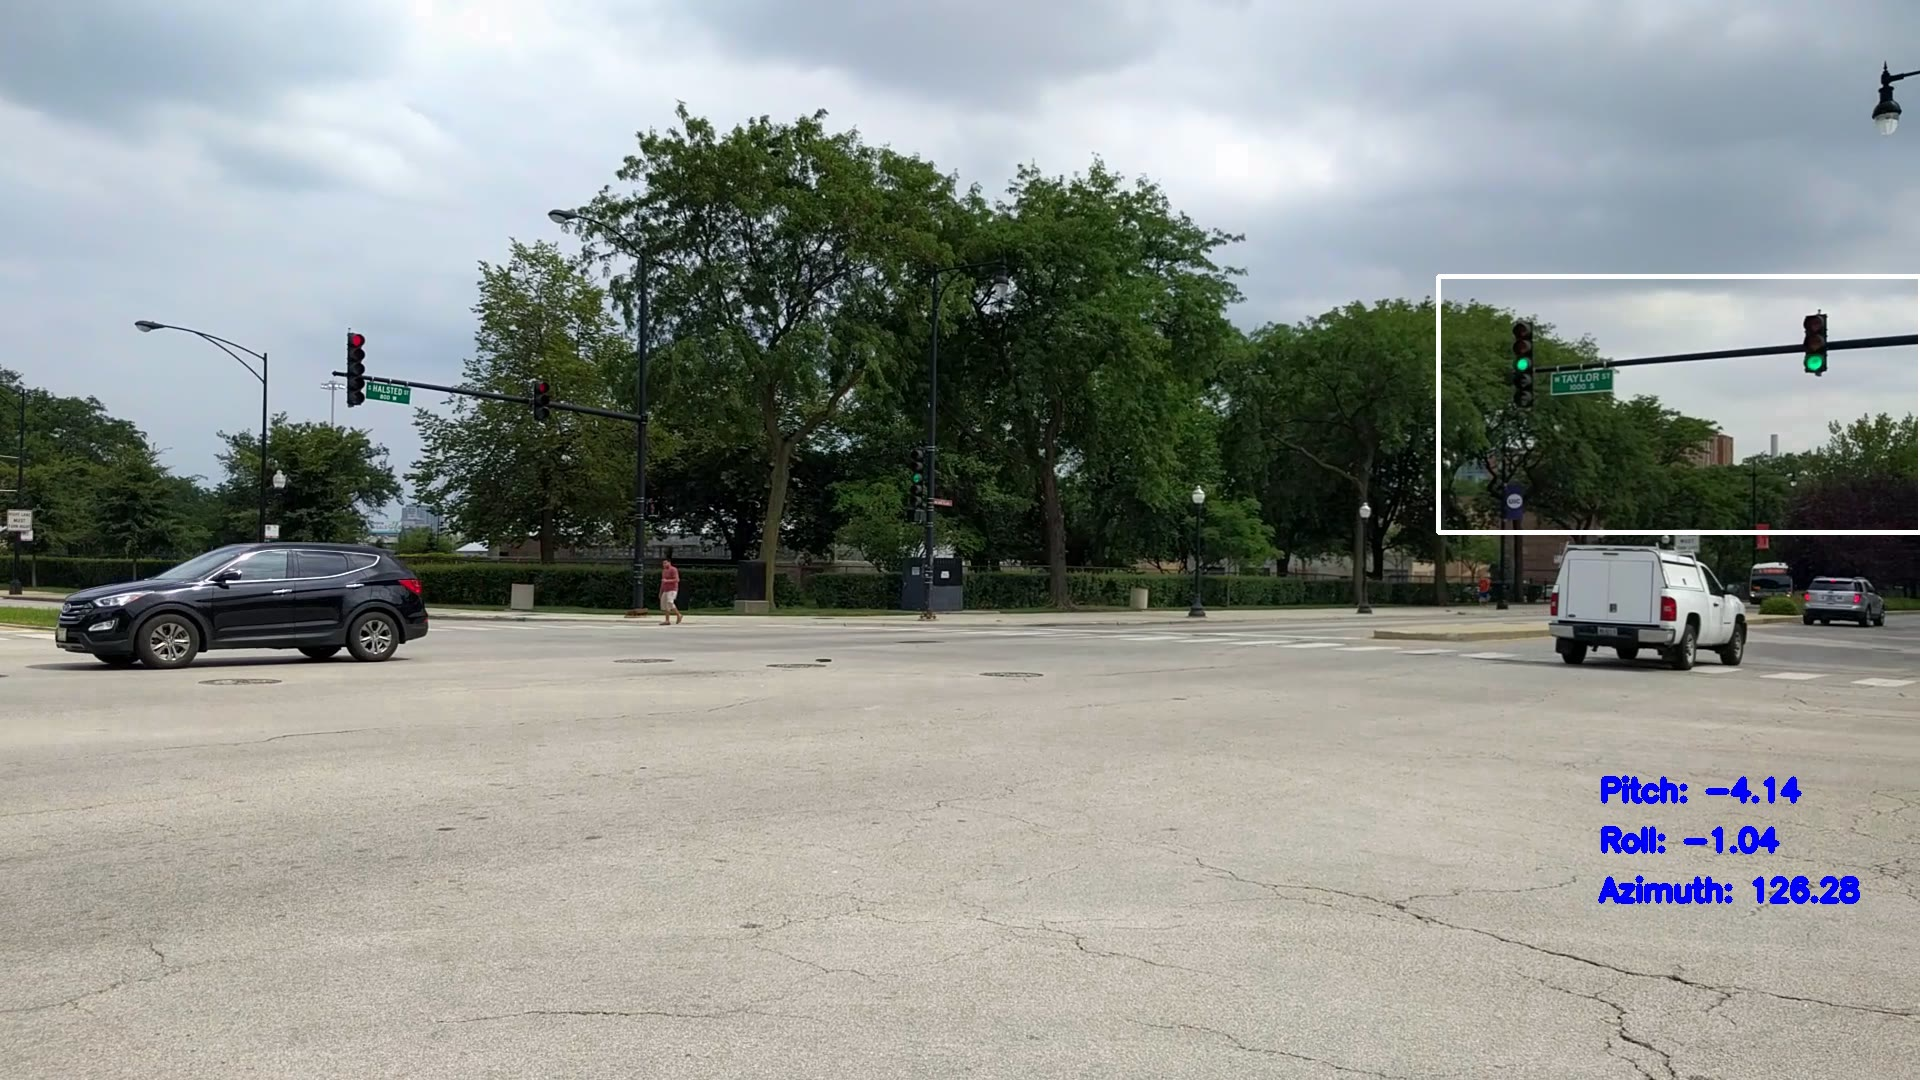
\includegraphics[width=4.2in]{images/rec_mv2.jpg}}

\caption{ROI movement with the change of sensor data.}
\label{f:rec_mv}
\end{figure*}


With the successful detection, our region of interest again changes with the light position and pitch and azimuth value.
For unsuccessful detection, ROI enlarged until it process the full frame and then go to the next frame to detect traffic light.
And this process is continuing to every frame.

\begin{figure*}[!ht]
\centering
\subfloat {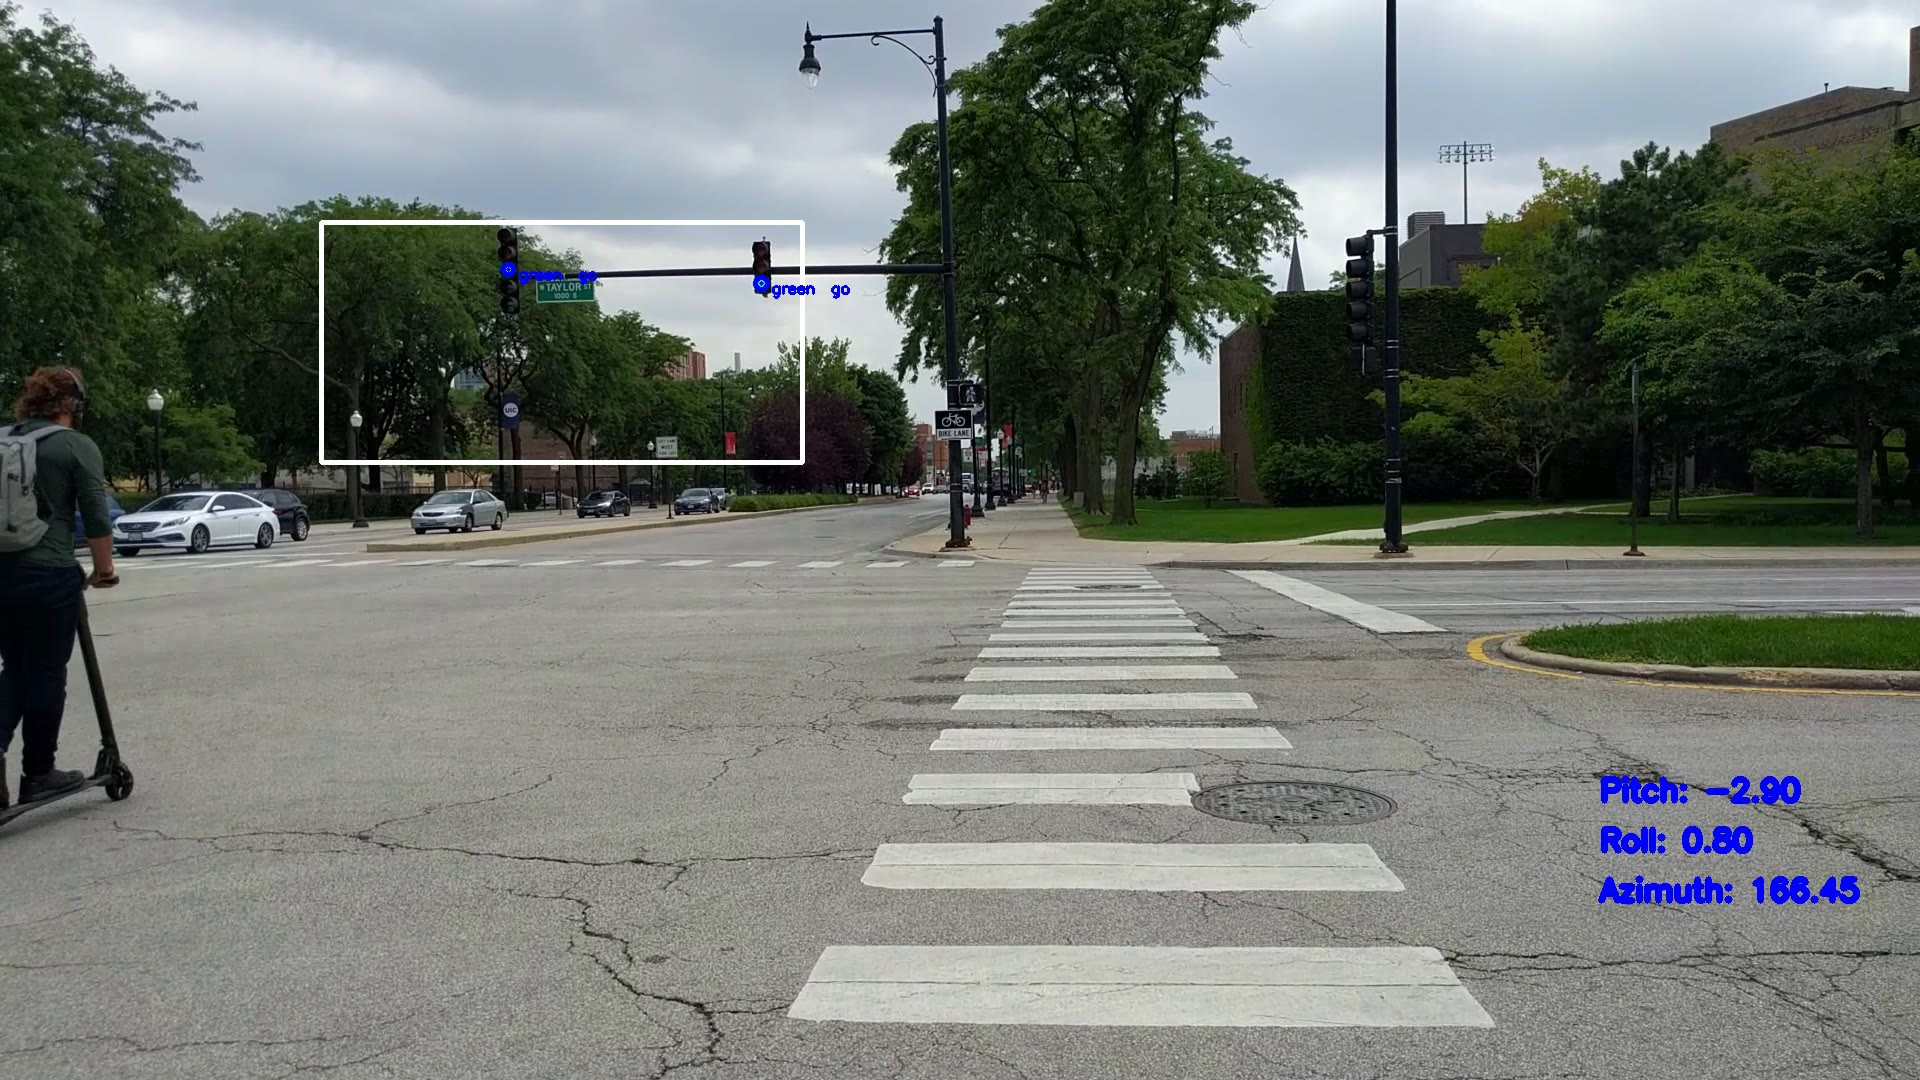
\includegraphics[width=4.2in]{images/rec_enl.jpg}}\\
\subfloat {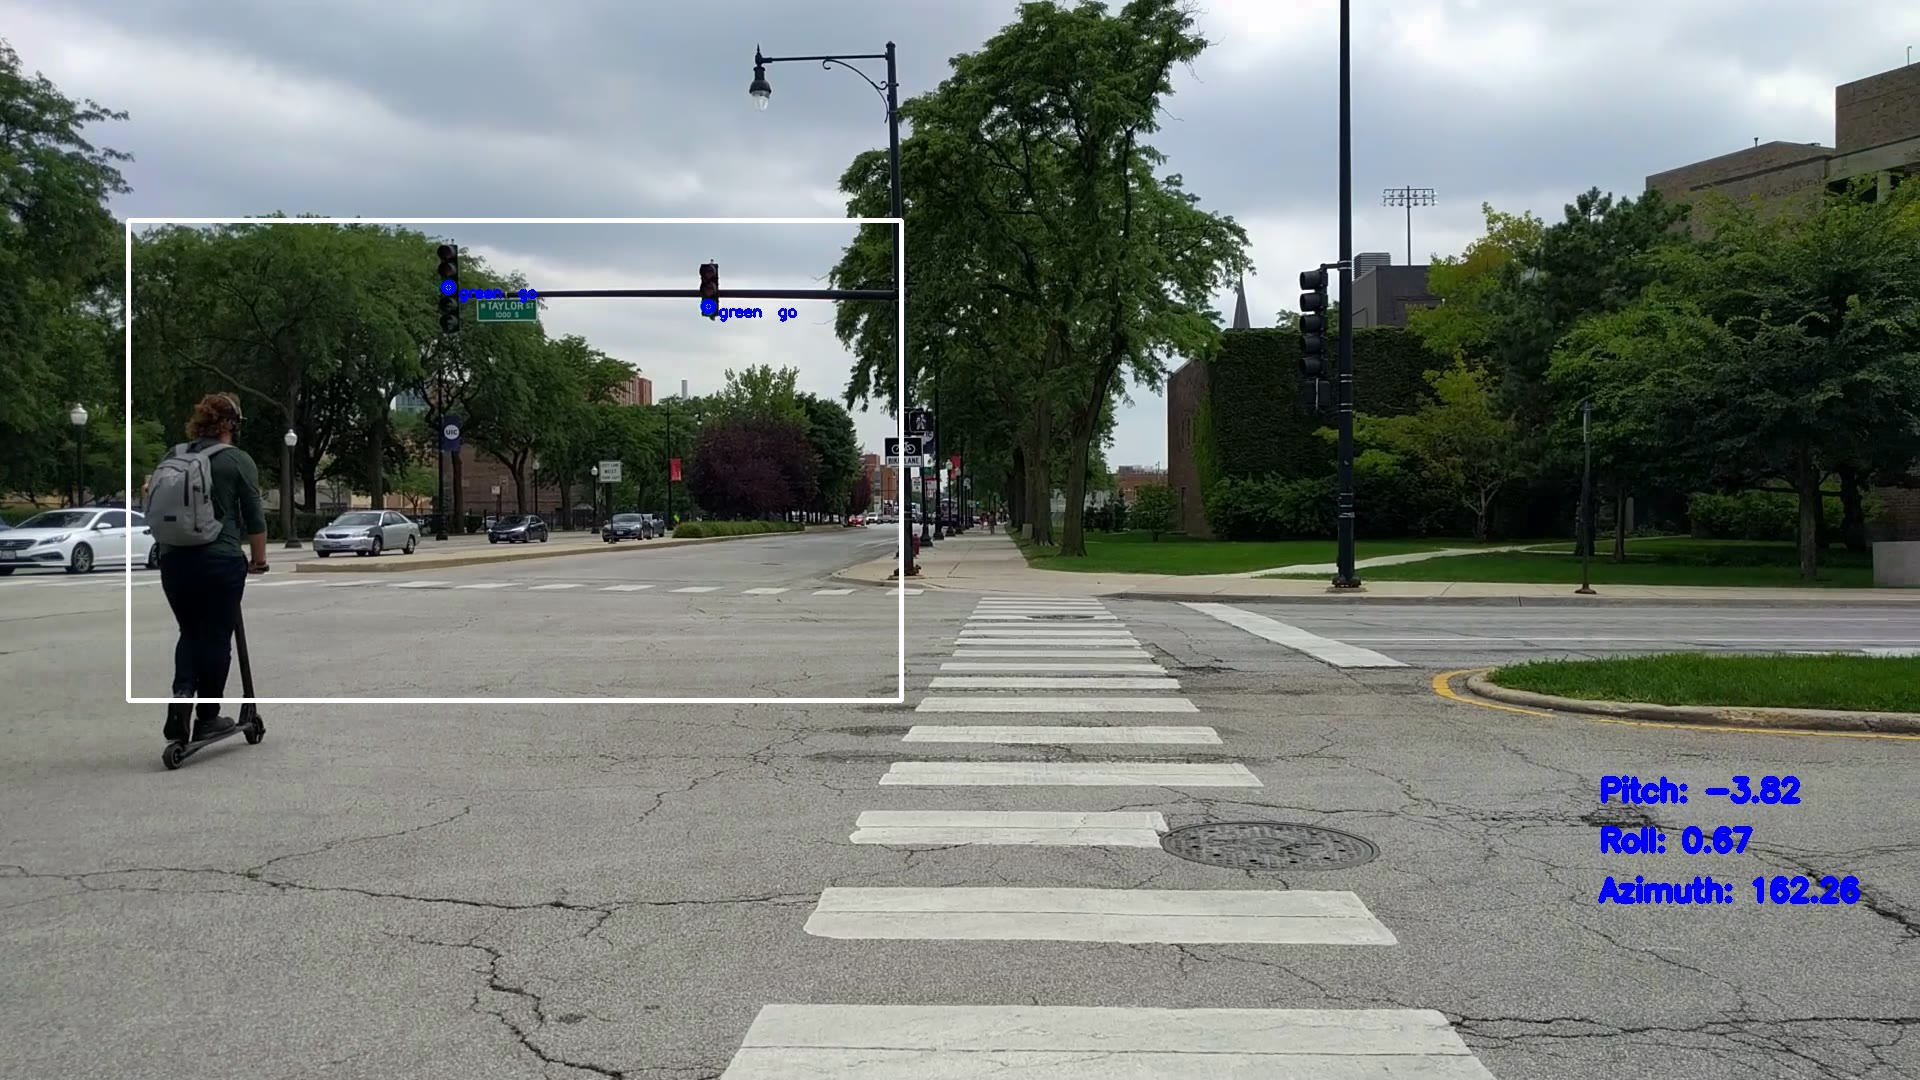
\includegraphics[width=4.2in]{images/rec_enl1.jpg}}

\caption{Enlarged ROI to detect traffic light successfully.}
\label{f:rec_enl}
\end{figure*}



\chapter{Evaluation}
\label{c:evalu}

In this chapter, we present the end-to-end evaluation of our system.
At first, we discuss the evaluation datasets and ground truth annotation.
Next, we present the quantitative results for both computation time and accuracy.
Finally, we conclude this chapter with evaluation of our system using a public dataset.

\section{Evaluation datasets}
\label{s:eval}
To our best knowledge, there is not much research on sensor fusion in the context of traffic light detection, especially for pedestrian navigation. 
As a result, we did not find public datasets combining traffic lights video and inertial sensor data. 
Hence, we collected our own ground truth data using an Android app.
% \todo{refer section or fig with the screenshot}.
We walked across several street crossings and recorded both video and sensor data simultaneously in various lighting conditions. 
For example, \ref{f:dataset} shows video frames for both sunny and cloudy days. 
Here, we present our results for several 300 feet long walks.  
At the end of this chapter, we present an approximate evaluation of a public dataset that does not have sensor data. 
However, we emulate the effect of sensors by manual selection of a subpart of a video frame. 

\begin{figure}[!ht]
\centering
\subfloat[Sunny] {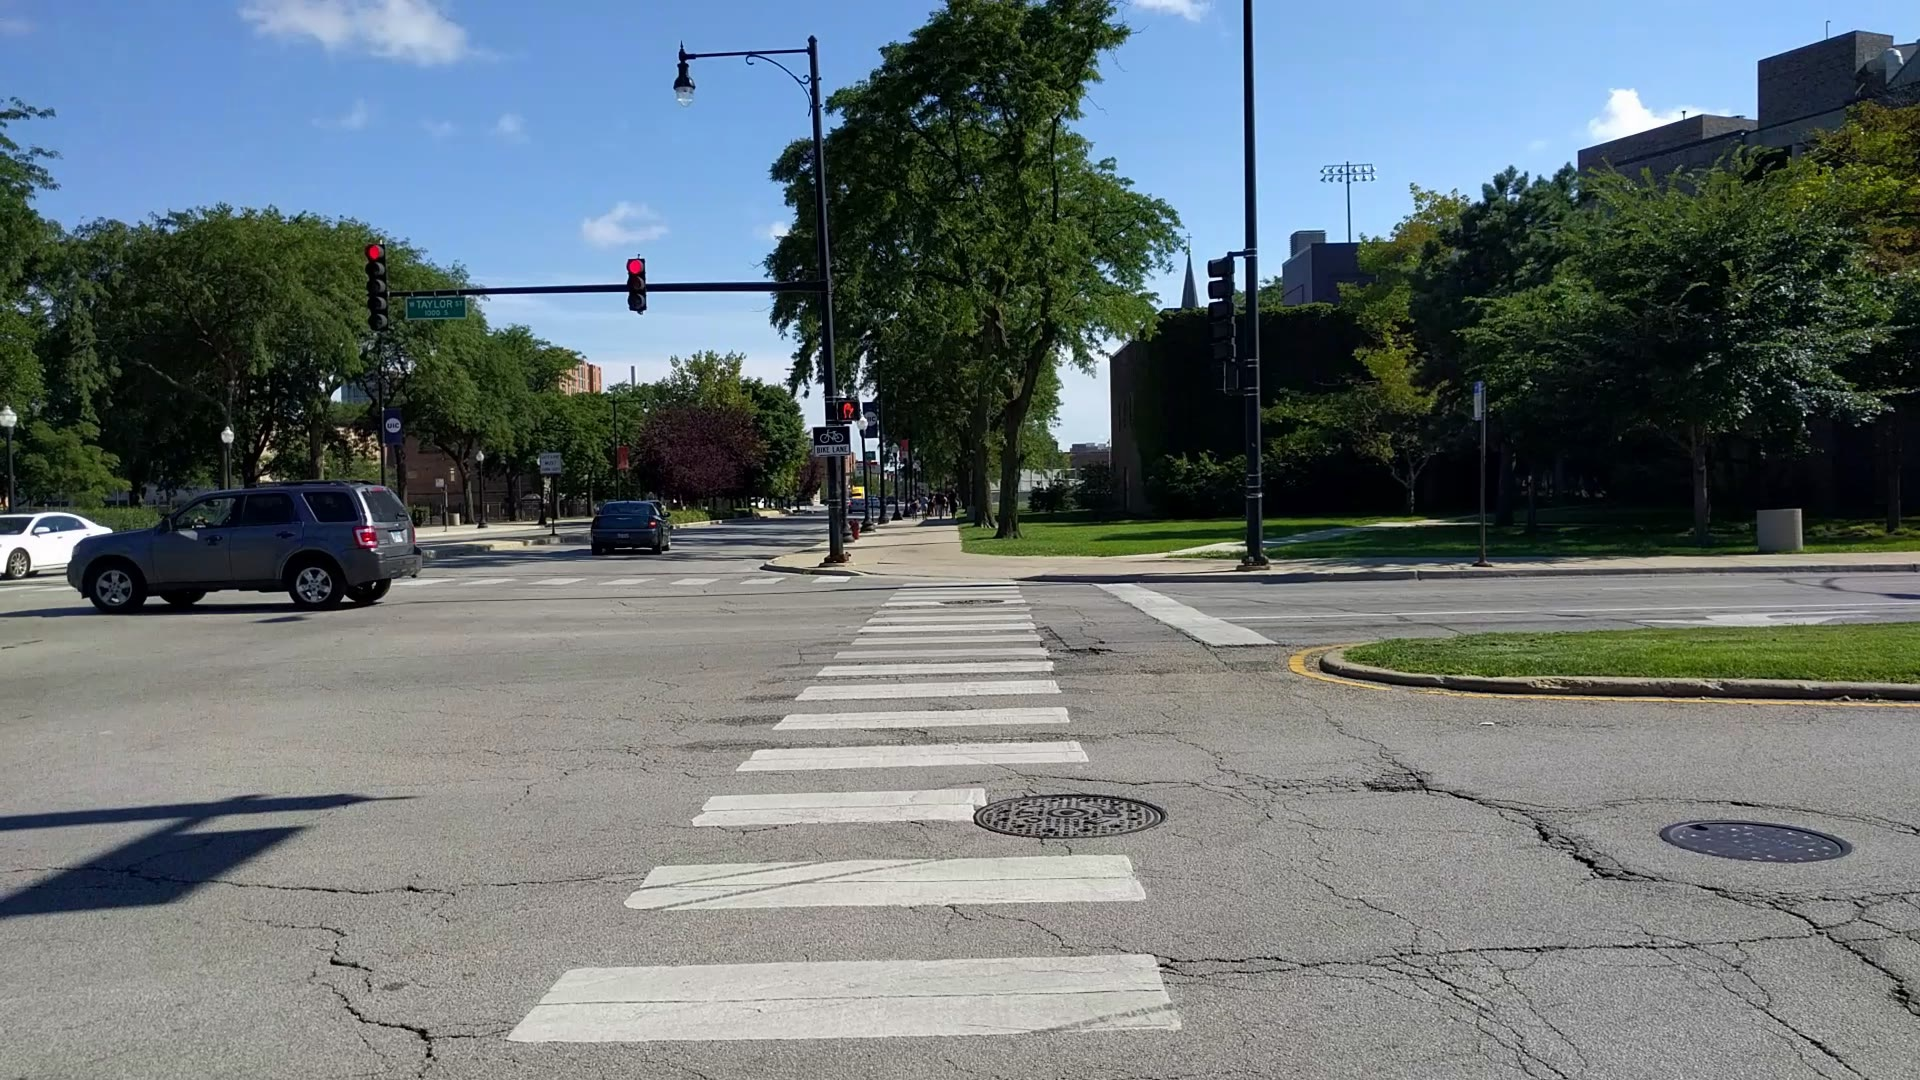
\includegraphics[width=3.1in]{images/sunny.jpg}}
\hfill
\subfloat[Cloudy] {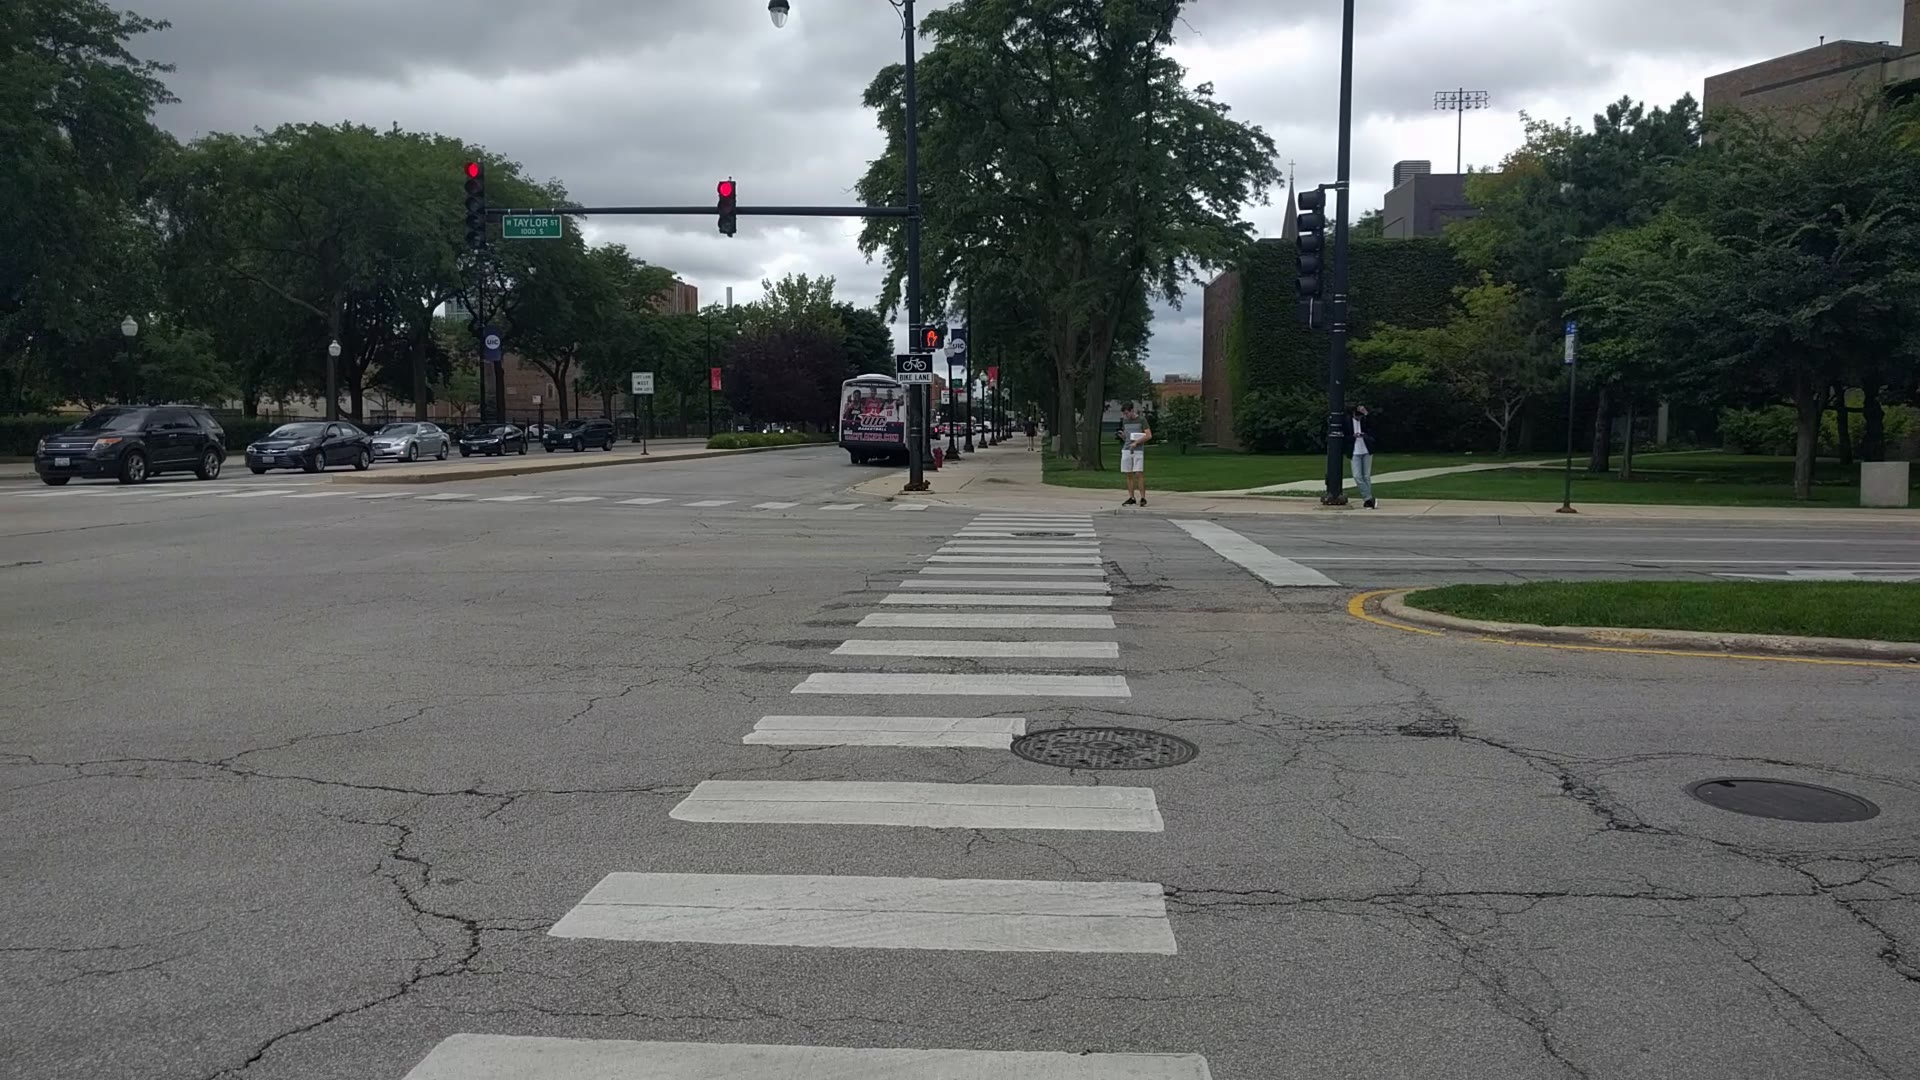
\includegraphics[width=3.1in]{images/cloudy.jpg}}
\caption{Scene variation of recorded video.}
\label{f:dataset}
\end{figure}

\ref{t:dataset} shows the total no of frames and time duration of our dataset.

\begin{table}[h!]
  \centering
  \caption{Description of the dataset.}
  \label{t:dataset}
  \begin{tabular}{  l  c  r  }   
    Name & Frame Count & Time Duration \\
    \hline
    Walk with sensor movement-Sunny day & 5905 & 3 mins 16 secs  \\
    Walk with sensor movement-Cloudy day & 6205 & 3 mins 26 secs \\
    Walk regular movement & 6022 & 3 mins 20 secs \\
    Static with sensor movement & 1810 & 1 min \\
    \hline
  \end{tabular}
\end{table}

\section{Annotation}
We need the ground truth for traffic light positions on video frames in order to measure our system performance quantitatively.
Accordingly, we annotate the traffic light's positions manually by drawing a rectangle around the traffic lights at each video frame.
During annotation, we record the type of the traffic lights (i.e., red or green) and their positions with a bounding box.

\ref{f:annotate} shows the interface for manual annotation.
The green box provides the location of the traffic light and we annotate 0 for a red traffic light and 1 for a green traffic light.

\begin{figure}[h!]
\centering
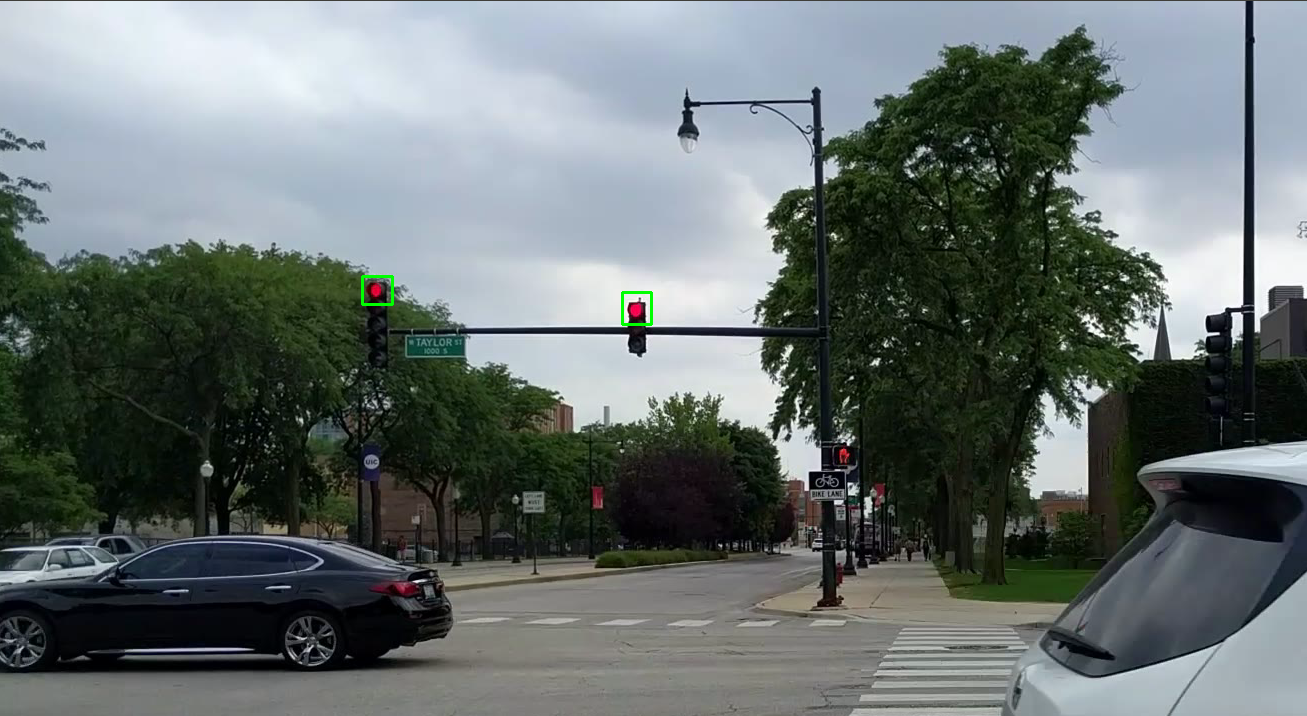
\includegraphics[width=5.2in]{images/annotation.png}
\caption{Interface for manual annotation.}
\label{f:annotate}
\end{figure}


\section{Computation time}
We collected data at different times of the day as we discussed in \ref{s:eval}.
In this section, we discuss the computation time of these datasets with and without the sensor fusion.

\subsection{Frame processing time}
\ref{f:cdf_time} shows the computation time CDF for video frames for walking dataset with regular movement described in \ref{t:dataset}.
It shows that the median of the computation time without the sensor data and without the heuristic filters is 106ms.
On the other hand, the median computation time with the sensor and without heuristic filters is 13ms.
This is an improvement of 8.15x.
The median computation time with sensor and heuristic filters is 19ms.
There is a slight increase in frame processing time with the heuristic filters, but this is worthwhile as we false detection rate reduces significantly with the heuristic filters.  
We discuss more about the accuracy and false detections in Section \ref{s:acc}

\begin{figure}[h!]
\centering
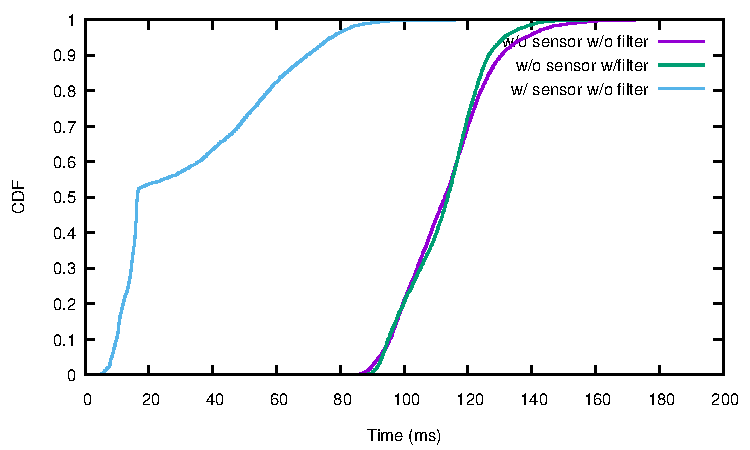
\includegraphics[width=5.2in]{plots/sunny_cdf_time.pdf}
\caption{CDF of frame computation time for walking dataset in sunny weather.}
\label{f:cdf_sunny}
\end{figure}

\ref{f:cdf_sunny} shows the CDF of the video frame computation time for walking dataset with sensor fusion on a sunny day.
It shows that the median computation time without the sensor is 107ms and with the sensor is 13ms, resulting in an improvement of 8.23x.


\subsection{Subimage processing time}
Processing a subpart of a video frame significantly reduces the computation time. 
We select a Region-Of-Interest (ROI) area within a frame with the sensor hints.
However, the ROI predicted from the sensor hints can be incorrect and we gradually increase the area of the rectangle.
We discussed the details about this in \ref{s:roi}.


\ref{f:recarea} shows the computation time with the increase of the ROI area in video frames.
It shows that the computation time increases as the area of the rectangle get larger.
For the same area, if the number of candidate pixels is high or the detected circle count is high then computation time can be also high.

\begin{figure}[h!]
\centering
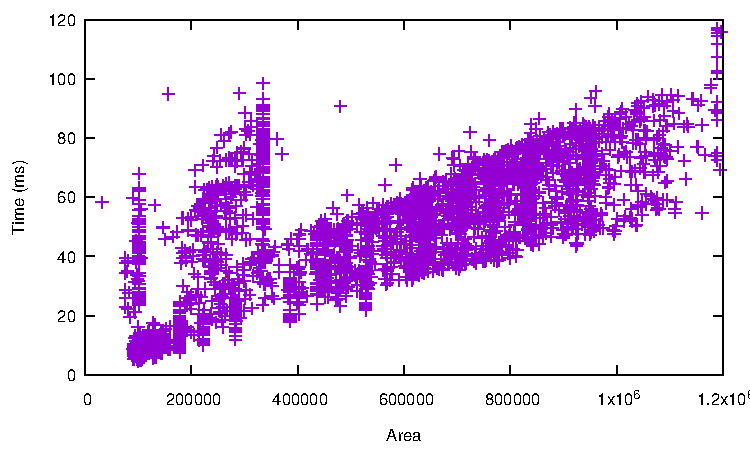
\includegraphics[width=5.2in]{plots/sunny_recarea.pdf}
\caption{Computation time with the increase of the rectangle area.}
\label{f:recarea}
\end{figure}



\subsection{Time for heuristic filtering}
We use a heuristic filter to reduce false positive in traffic light detection as we discuss at \S\ref{s:filter}.
The computational cost of the heuristic filter is very small.

\begin{figure}[h!]
\centering
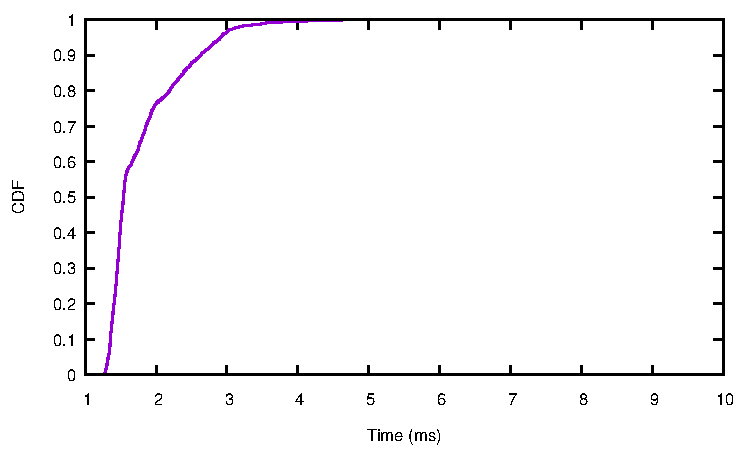
\includegraphics[width=5.2in]{plots/sunny_cdf_filter.pdf}
\caption{CDF of computation time for the heuristic filter.}
\label{f:cdf_fil}
\end{figure}

\ref{f:cdf_fil} shows the computation time of the heuristic filter that we discuss at \S\ref{s:filter}.
The computation time depends on the number of circles detected on the frame.
If circle count is high, filtering need for all of these circles, so computation time gets higher.
\ref{f:cdf_fil} shows that the median computation time is 1.5 ms for the filtering. 


\begin{figure}[h!]
\centering
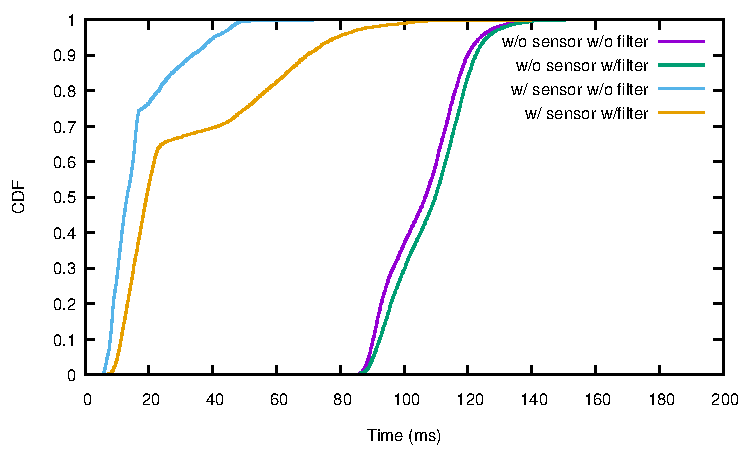
\includegraphics[width=5.2in]{plots/walk_cdf_time.pdf}
\caption{CDF of frame computation time.}
\label{f:cdf_time}
\end{figure}



\section{Traffic lights detection accuracy}
\label{s:acc}
To demonstrate the robustness of the various traffic light scenarios, we recorded video at different lightening condition such as cloudy and sunny and at the different time of the day.
We walked along several crosswalks of few streets and the route had a total of 16 traffic lights.

\subsection{Confusion matrix}
\ref{t:con_nocrp} shows the confusion matrix for the traffic light decision when we do not consider the sensor hints of the smartphone.
\ref{t:con_crp} shows the confusion matrix considering the sensor hints in the same dataset.

\begin{table}[h!]
  \centering
  \caption{Confusion Matrix without sensor hints for static movement dataset.}
  \label{t:con_nocrp}
  \begin{tabular}{  l | c | c | r }
   
     & Detected Red & Detected Green &  \\
    \hline
    Actual Red & 828 & 1 & 99.88\% \\
    \hline
    Actual Green & 54 & 509 & 90.41\% \\
    \hline
    & 93.88\% & 98.8\% & 96.05\% \\
    
  \end{tabular}
\end{table}

\begin{table}[h!]
  \centering
  \caption{Confusion Matrix with sensor hints for static movement dataset.}
  \label{t:con_crp}
  \begin{tabular}{  l | c | c | r }
   
     & Detected Red & Detected Green &  \\
    \hline
    Actual Red & 909 & 1 & 99.89\% \\
    \hline
    Actual Green & 36 & 524 & 93.57\% \\
    \hline
    & 96.19\% & 99.81\% & 97.48\% \\
    
  \end{tabular}
\end{table}

These results show that the use of sensor hints increases the accuracy of the red light detection and reduces false detection of green lights.


\subsection{Detection and misdetection rate for traffic lights}
\ref{f:tp_stat} shows the detection rate for the red and green state of the traffic lights.
It shows that using the sensor hints detection rate for red lights increases from 86\% to 96\% and the detection rate for green lights increases 96\% to 99\%.

\begin{figure}[h!]
\centering
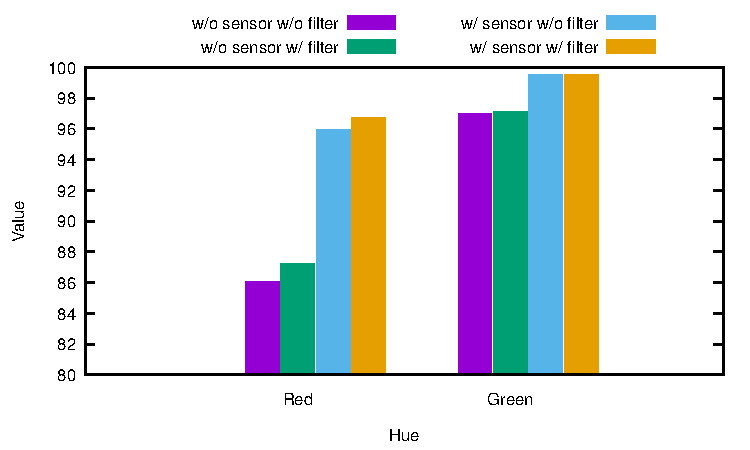
\includegraphics[width=5.2in]{plots/bar_tp.pdf}
\caption{Detection rate for static movement dataset.}
\label{f:tp_stat}
\end{figure}

\ref{f:fp_stat} shows the misdetection rate for the red and green state of traffic lights.
Left one is the false positive detection and the right one is the false negative detection for the traffic light detection.
Here, the false positive count is reduced significantly and false negative is zero.

\begin{figure}[!ht]
\centering
\subfloat[] {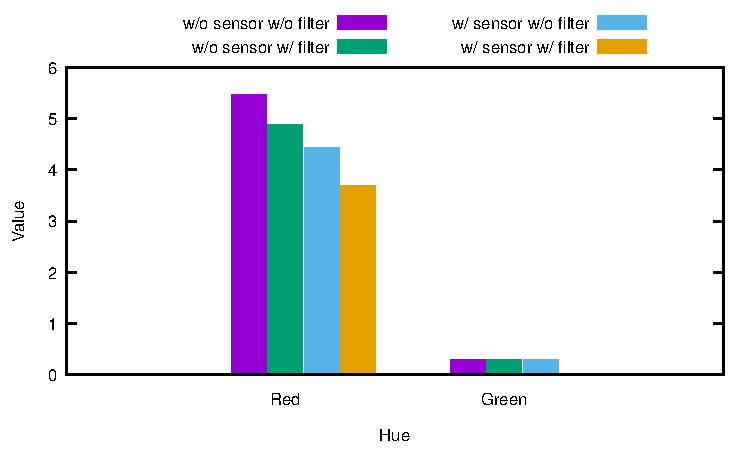
\includegraphics[width=5.2in]{plots/bar_fp.pdf}}

\subfloat[] {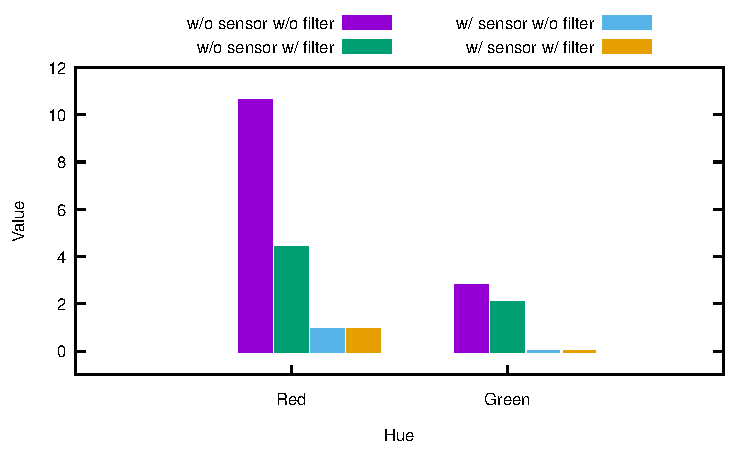
\includegraphics[width=5.2in]{plots/bar_fn.pdf}}
\caption{Misdetection rate for static movement dataset.}
\label{f:fp_stat}
\end{figure}

\ref{t:acc_stat} shows the accuracy rate for the static with sensor movement dataset.
It shows that the accuracy increases from 89\% to 97\% with sensor hints.

\begin{table}[h!]
  \centering
  \caption{Accuracy for detection.}
  \label{t:acc_stat}
  \begin{tabular}{  l  c | r  }
   
     & without sensor & with sensor  \\
    \hline
    & 89.7313\% & 97.035\%  \\
    \hline
  \end{tabular}
\end{table}


\section{Evaluation of a public dataset}

\todo{need to add results here}

\section{Effect of video/image resolution}

\todo{\ref{f:vf_res} shows the computation time after changing video frames resolution.}

\begin{figure}[h!]
  \centering
  \vspace{2in}
  %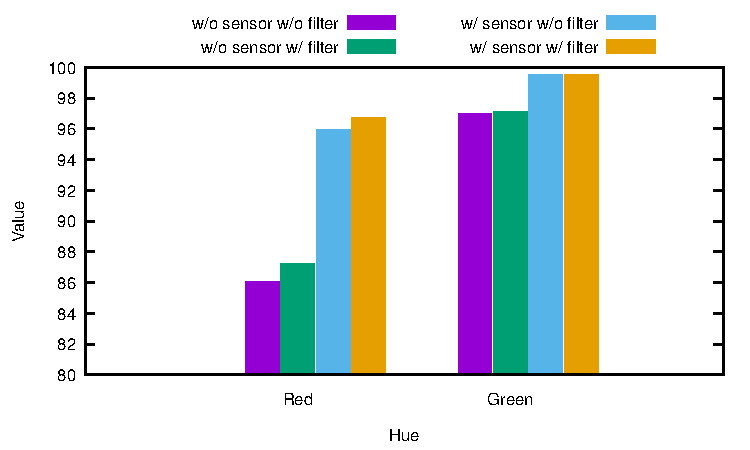
\includegraphics[width=5.2in]{plots/bar_tp.pdf}
  \caption{Effect of the computation time after changing video frames resolution.}
  \label{f:vf_res}
\end{figure}


\chapter{Conclusion}

In conclusion, in this dissertation, we presented a system that we developed to detect the traffic light with the sensor hints of the smartphones.
This system can be useful for the pedestrian navigation, especially visually impaired.
We combine the sensor fusion with the image processing to efficiently detect traffic light in a subframe.
Firstly, we predict and track the traffic lights in a video frame using the orientation of the smartphone.
The subframe selection depends on the prediction of traffic light position using the sensor hints from the smartphone.
The subframe processing provides us computation time improvement and better accuracy.
We get in an order of magnitude improvement of computation time on average and our misdetection rate is significantly reduced.
In our system, although we use the model-based computer vision technique to detect the traffic light using the color and shape information.
Learning-based technique can also be combined with our algorithm with the sensor hints which can provide improved result with the improvement of the computation time.
%Nowadays many learning-based techniques are used to detect the traffic light that provides a  significant result.
%Finally, overall results may be improved if our traffic light detection algorithms with the sensor hints are combined with the learning-based algorithm for detecting traffic light states.




\bibformb
%\bibliographystyle{abbrv}
\bibliography{ref}

\newpage
\vita
\singlespace
\begin{list}
{}
{\setlength
   {\labelwidth}{1in}
    \setlength{\leftmargin}{0.8in}
    \setlength{\labelsep}{.2in}
    \setlength{\itemsep}{0.2in}
    \setlength{\rightmargin}{\leftmargin}}

\item[Name\hfill] Nishat Anjum Khan

\item[Education\hfill] M.Sc., Electrical and Computer Engineering, University of Illinois at Chicago, 2017.

B.S., Electrical and Electronics Engineering, Bangladesh University of Engineering and Technology, 2014.

\item[Publications\hfill] 
A.B.M. Musa, James Biagioni and Jakob Eriksson, “Trading Off Accuracy, Timeliness, and Uplink Usage in Online GPS Tracking,” in IEEE Transactions on Mobile Computing (TMC), vol. 15, no. 8, pp. 2124--2136, Aug. 1 2016.

James Biagioni, A.B.M. Musa, and Jakob Eriksson, “Thrifty Tracking: Online GPS Tracking with Low Data Uplink Usage”, In Proceedings of the 21st ACM SIGSPATIAL International Conference on Advances in Geographic Information Systems (SIGSPATIAL’13). ACM, New York, NY, USA, 496--499.

A.B.M. Musa and Jakob Eriksson. “Tracking unmodified smartphones using Wi-Fi monitors”, In Proceedings of the 10th ACM Conference on Embedded Network Sensor Systems (SenSys ’12). ACM, New York, NY, USA, 281--294.

A.B.M. Musa, Jakob Eriksson, “Demo: WiFlow: Real-time Travel Time Estimation using Wi-Fi Monitors”, In Proceedings of the 9th ACM Conference on Embedded Networked Sensor Systems (SenSys ’11). ACM, New York, NY, USA, 429--430.

A.B.M. Musa, Jakob Eriksson, “On-Demand, Deploy-Anywhere Wi-Fi Diagnostics”, Demo In Proceedings of the sixteenth annual international conference on Mobile computing and networking (MobiCom ’10), ACM, New York, NY, USA.


\item[Awards\hfill]
Dean’s List merit scholarship awarded by the dean of EEE faculty (2009--2014)

Educational Board Scholarship awarded by Government of Bangladesh (2008--2014)

Educational Board Scholarship awarded by Government of Bangladesh (2006--2008)

Junior Board Scholarship awarded by Government of Bangladesh (2005--2006)

\item[Service\hfill] 

Member of Teacher Association at Daffodil University, Bangladesh (2014--2015)

Organizer at countrywide EEE Undergraduate Project Workshop (2009, 2011)

Volunteered at IEEE WIE 20 th anniversary summit - 2014 in Bangladesh.

\end{list}

%% \begin{center}
%%  \Large{Tim Merrifield}
%%  \end{center}.
%%  \section*{Education}
%%  Bachelor of Science in Computer Science - Ohio University, Athens Ohio (2004))

%% \section*{Research Experience}
%% \begin{itemize}
%% \item \textbf{BITS Networking Lab, UIC}: Research Assistant ( May 2009 - Present)
%% \end{itemize}

%% \section*{Professional Experience}
%% \begin{itemize}
%% \item \textbf{Argonne National Laboratory, Decision and Information Sciences Division}: Software Engineer (January 2010 - Present )
%% \item \textbf{ShopLocal LLC}: Software Engineer (March 2005 - December 2009 )
%% \end{itemize}




%% \renewcommand{\baselinestretch}{1.0}
%% \linespread{1.0}
%% \noindent \begin{tabular}{@{} l l}

%%  \textbf{Education}  & Ph.D., Computer Science, University of Illinois at Chicago, 2017. \\
%%      & B.S., Computer Science, Bangladesh University of Eng. and Tech., 2008. \\
%%      & \\
%%  \Large{Dissertation}    & ``Title of Dissertation" \\
%%     & \parbox{5.0in}{Short description/summary of research and estimation techniques. This can be several lines long because of the paragraph box.}\\
%%     & \\
%%  \Large{Research}    & \textbf{Department, University} \\
%%      & Postdoctoral Research Associate \\
%%      & Project: Title of Research \\
%%      & \\
%%   \Large{Teaching}   & \textbf{Department, University} \\
%%      & Instructor, Fundamentals of the Global Economy, 2016 \\
%%      & \\
%%      &\textbf{Department, University} \\
%%      & Job Title, Course Name, 2014-2015 \\
%%      & Job Title, Course Name, 2012-2014 \\
%%      & \\
%%      & \textbf{Department, University} \\
%%      & Job Title, Course Name, 2013 \\
%%      & Job Title, Course Name, 2013 \\
%%      & \\
%%  \Large{Awards and }    & \textbf{Graduate Student Teacher of the Year, Department} \\
%%   \Large{Fellowships}   & Course Name, 2014-2015 \\
%%      & \\
%%      & \textbf{Fulbright Scholarship} \\
%%      & City, Country, 2006-2009 \\
%%      & \\
%%   \Large{Languages}   & English (native), German (advanced) \\
%% \Large{and Skills}    & Stata, \LaTeX, Eviews, Mathematica  \\
%% \end{tabular}





%% %\begin{table}
%% \begin{tabularx}
%% %\centering
%% \begin{tabular}{\linewidth}{l X}

%% \textbf{Name} & ABM Musa \\

%% \textbf{Education}  &  PhD, Computer Science, University of Illinois at Chicago, 2017  \\
%% ``" & BS, Computer Science, Bangladesh University of Eng. and Tech., 2008  \\

%% \textbf{Publications} & A.B.M. Musa, James Biagioni and Jakob Eriksson, “Trading Off Accuracy, Timeliness, and Uplink Usage in Online GPS Tracking,” in IEEE Transactions on Mobile Computing, vol. 15, no. 8, pp. 2124-2136, Aug. 1 2016.

%% \end{tabularx}
%% %\end{tabular}
%% \label{tab:vita}
%% \end{table}


\end{document}
